\ifnum\aluno=1
\renewcommand\chapterillustration{./abertura-computacional}
\else
\renewcommand\chapterillustration{./abertura-computacional-professor}
\fi

\renewcommand\chapterwhat{Pensamento computacional e noções básicas de linguagem de programação.
}
\renewcommand\chapterbecause{Os computadores estão presentes em quase todas as atividades humanas na atualidade e, por isso, desenvolver o pensamento computacional e conhecer noções básicas de linguagens de programação pode ser fundamental para sua vida profissional, trajetória acadêmica e participação efetiva na sociedade.
} 
\chapter{Pensamento Computacional}
\label{computacional-chap}

\mbox{}\thispagestyle{empty}\clearpage

\thispagestyle{empty}

\begin{center}
Projeto: LIVRO ABERTO DE MATEMÁTICA

\noindent \begin{tabular}{lcccr}

\includegraphics[scale=.15]{impa}& \quad\quad& 
\includegraphics[width=3cm]{logo} & \quad\quad& 
\includegraphics[scale=.24]{obmep} 
\end{tabular}
\end{center}

\vspace*{.3cm}

Cadastre-se como colaborador no site do projeto: \url{umlivroaberto.org}



% \begin{center}
%   \includegraphics[width=2cm]{canvas}
% \end{center}

\begin{tabular}{p{.15\textwidth}p{.7\textwidth}}
Título: & Pensamento Computacional\\
\\
Ano/ Versão: & 2021 / versão 0.1 de \today\\
\\
Editora & Instituto Nacional de Matem\'atica Pura e Aplicada (IMPA-OS)\\
\\
Realização:& Olimp\'iada Brasileira de Matem\'atica das Escolas P\'ublicas (OBMEP)\\
\\
Produção:& Associação Livro Aberto\\
\\
Coordenação: & Fabio Simas, \\
			&  Augusto Teixeira (livroaberto@impa.br)\\
\\
  Autores: & Leonardo Barichello\\
\\
Colaboração: & \\
\\
Revisor: & Diego Lieban \\
		 & Larissa Monzon \\
		 & Kátia Rocha
\\
Design: & Andreza Moreira (Tangentes Design) \\
\\
  Ilustrações: & --- \\ 
\\
Gráficos: & ---\\
\\
  Capa: & Foto de Pankaj Patel, no Unsplash \\
  		& https://unsplash.com/photos/yEAOfWSdzgM \\

\end{tabular}
\vspace{.5cm}



\begin{figure}[b]
\begin{minipage}[l]{5cm}
\centering

{\large Licença:}

  
\includegraphics[width=3.5cm]{cc-by-nc-sa}
\end{minipage}\hfill
\begin{minipage}[c]{5cm}
\centering
{\large Desenvolvido por}


\includegraphics[width=2.5cm]{logo-associacao.jpg}
\end{minipage}
\begin{minipage}[r]{5cm}
\centering

{\large Patrocínio:}
  \vspace{1em}
  
\includegraphics[width=3.5cm]{itau}
\end{minipage}
\end{figure}

\mainmatter

\begin{apresentacao}{Introdução ao professor}
\subsection{Pensamento computacional na BNCC}

A versão atual da BNCC traz o desenvolvimento do pensamento computacional como um dos objetivos relacionados à área de Matemática desde os Anos Finais do Ensino Fundamental até o Ensino Médio. Essa expressão não aparece nem nas competências nem nas habilidades, mas é mencionada diversas vezes ao longo das discussões propostas no documento, sempre nas seções sobre Matemática.

Em geral, essas menções sugerem que o desenvolvimento do pensamento computacional deve ser visto como uma contribuição desejável à Matemática nesses níveis de ensino:

\begin{quote}
Outro aspecto a ser considerado é que a aprendizagem de Álgebra, como também aquelas relacionadas a Números, Geometria e Probabilidade e Estatística, podem contribuir para o desenvolvimento do pensamento computacional dos alunos \citep[BNCC,][p. 271]{BNCC2018}
\end{quote}

Embora essa recomendação ocorra em diversos momentos do documento, uma busca por ``pensamento computacional"{} nas habilidades apresenta nenhum exemplo objetivo, sendo possível apenas identificar termos relacionados a essa temática, como fluxogramas e algoritmos, em algumas habilidades de Matemática (e apenas de Matemática) do Ensino Fundamental e do Ensino Médio. No caso do Ensino Médio, as duas habilidades que fazem menções dessa natureza, e que serão cobertas por este módulo, são:

\begin{habilities}{EM13MAT315}
Reconhecer um problema algorítmico, enunciá-lo, procurar uma solução e expressá-la por meio de um algoritmo, com o respectivo fluxograma.

\tcbsubtitle{EM13MAT405}

Utilizar os conceitos básicos de uma linguagem de programação na implementação de algoritmos escritos em linguagem corrente e/ou matemática.
\end{habilities}

Mas então, o que seria o pensamento computacional?

Esse termo é associado a um crescente movimento mundial de incorporação da computação a currículos escolares não apenas como ferramentas pontuais para ensino e aprendizagem de alguns conceitos, mas como um disciplina ou um conjunto de habilidades mais amplo que esteja relacionado ao mundo digital \citep{raabe2020}.

Mas para nos ajudar a entender de forma mais concreta, vamos considerar o currículo de referência em "Teconologia e Computação"{} proposto pelo Centro de Inovação para a Educação Brasileira (CIEB), disponível em curriculo.cieb.net.br/curriculo. Essa proposta, divide o currículo em três grandes eixos: Cultura Digital, Tecnologia Digital e Pensamento Computacional. Para este terceiro eixo, é dada a seguinte definição:
\begin{quote}
Pensamento Computacional refere-se à capacidade de resolver problemas a partir de conhecimentos e práticas da computação, englobando sistematizar, representar e analisar.
\end{quote}

Além disso, a proposta divide o Pensamento Computacional em 4 conceitos: Abstração, Algoritmos, Decomposição e Reconhecimento de Padrões.

Embora o currículo de referência do CIEB seja muito claro e completo em termos de organização, inter-relações e práticas, do ponto de vista de um professor de Matemática, a definição e os quatro conceitos soam como habilidades que já são ou poderiam ser desenvolvidas em aulas de matemática, sem que houvesse necessidade de trazer este tal de pensamento computacional para o cenário.

A concepção que vamos desenvolver na próxima seção busca justamente salientar o que o pensamento computacional pode trazer de novo para um professor de matemática no Ensino Médio.

\subsection{Pensamento computacional no Livro Aberto de matemática}

Vários são os autores que buscam definir o que é pensamento computacional \citep{shute2017} e é comum entre eles o reconhecimento de que há uma grande intersecção entre as habilidades e conceitos cobertos por este termo e as habilidades e conceitos cobertos pelo que poderíamos chamar de "pensamento matemático". Entretanto, um elemento que se destaca como exclusivo ao universo do pensamento computacional é o foco em processos de resolução de problemas.

Enquanto em Matemática o foco da atividade usualmente recai em dois objetos, a resolução de um problema ou a demonstração de um teorema, em computação o processo de resolução de um problema é o grande objeto de interesse. Nesse sentido, habilidades relacionadas a compreender e sistematizar esse processo ganham importância.

Isso será feito neste módulo através de um movimento que se inicia propondo problemas matemáticos e estendendo a discussão no sentido de mudar o foco progressivamente para o processo de resolução através de descrições textuais ou visuais e, em um momento posterior, na forma de um algoritmo descrito em uma linguagem de programação.

Tomemos como exemplo o seguinte cenário inspirado em uma questão da Olimpíada Brasileira de Informática:

\begin{quote}
O cometa Halley é um dos cometas de menor período do Sistema Solar, completando uma volta em torno do Sol a cada 76 anos; na última ocasião em que ele ficou visível do planeta Terra, em 1986, várias agências espaciais enviaram sondas para coletar amostras de sua cauda e assim confirmar teorias sobre suas composições químicas.
\end{quote}

A partir desse contexto, um professor de matemática colocaria questões como: Quando será a próxima passagem do cometa Halley? Uma pessoa que nascerá no ano 2500 terá a chance de avistar o cometa Halley pela primeira vez em que ano? Quantas vezes o cometa passará ao longo de todo o terceiro milênio?

Essas questões serão colocadas ao longo do módulo, mas complementadas por questões como essa:

\begin{quote}
Descreva como obter, a partir de um dado ano qualquer, qual é o próximo ano em que o cometa Halley será visível novamente do planeta Terra.
\end{quote}

Esse tipo de questão pode ser respondida de forma textual, com auxílio de notação matemática e fluxogramas ou como um algoritmo escrito em uma linguagem de programação, como mostrado na imagem abaixo.

\begin{figure}[H]
\centering

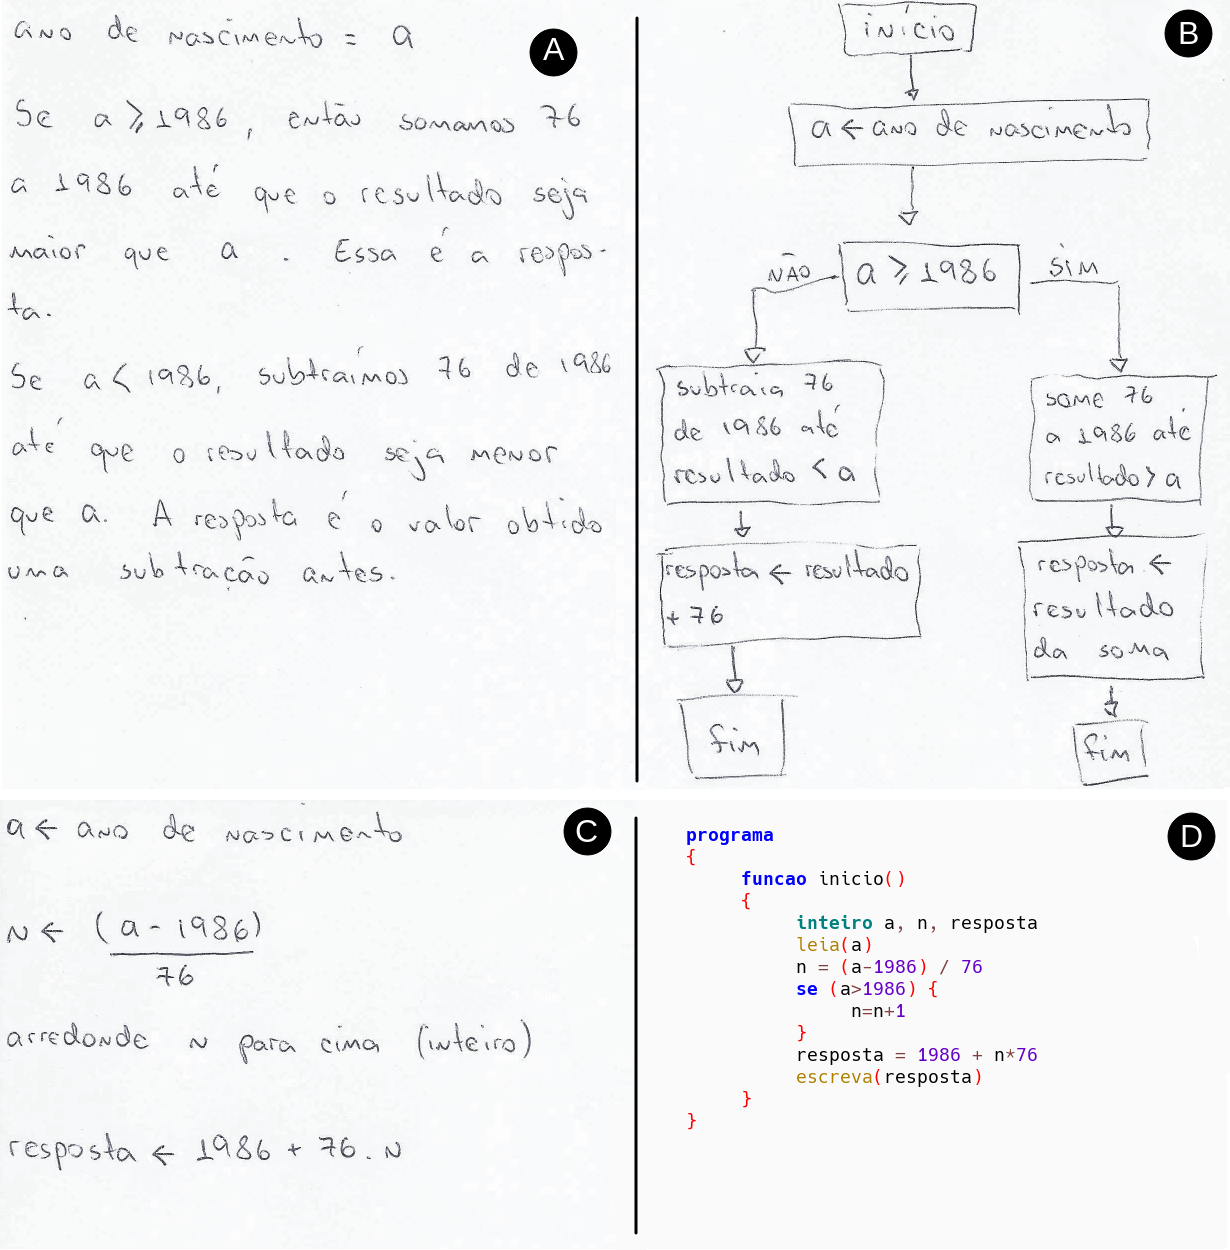
\includegraphics[width=\linewidth]{imagem_01}
\end{figure}

Ao longo do módulo, ao resolver um problema sob o ponto de vista computacional, esperamos que os estudantes vivenciem um movimento que se inicia com descrições textuais e notação matemática, passa por fluxogramas e se completa com uma linguagem de programação.

Entendemos que esse movimento cobre as duas habilidades relacionadas ao pensamento computacional colocadas na BNCC do Ensino Médio. Vale salientar que ambas enfatizam algoritmos (seja na forma de fluxograma ou em uma linguagem de programação) e isso justifica o foco que estamos dando a esse meio para promover o pensamento computacional neste módulo.

Entretanto, esse primeiro movimento representa apenas uma parte do que pretendemos: partindo de problemas matemáticos, propomos a discussão e criação de algoritmos que descrevam o processo de resolução destes problemas. A segunda parte faz o movimento contrário: uma vez que os estudantes saibam utilizar algoritmo para programar o computador para realizar certas tarefas, queremos que eles tenham a oportunidade de usar essa nova ferramenta para explorar novos problemas matemáticos.

Essa segunda parte demanda algum domínio sobre a nova ferramenta, por isso as atividades relacionadas a elas serão apresentadas mais adiante no módulo. Para ilustrar o tipo de questão que será explorada nessa segunda parte, pense em como você trabalharia uma questão de probabilidade envolvendo um jogo de dados, por exemplo, se você pudesse criar com os seus estudantes um simulador que permita repetir esse jogo milhares de vezes. Esse é o cenário que queremos criar na segunda parte deste módulo.

\subsection{A organização deste módulo}

A \textbf{primeira parte} desenvolve o primeiro movimento: resolver problemas matemáticos sob o ponto de vista computacional propondo atividades como o exemplo do cometa Halley dado anteriormente. Partimos de questões que seriam naturais em uma aula de matemática e gradualmente movemos o foco para o processo de resolução em si, concluindo com uma sistematização deste na forma de texto, fluxograma ou algoritmo escrito em uma linguagem de programação.

Para isso, além de introduzir esse novo modo de pensar ao estudante (seção 1 da primeira parte), também exploramos alguns conceitos básicos de linguagens de programação como variáveis (seção 2 da primeira parte), condicional (seção 3 da primeira parte) e repetição (seção 4 da primeira parte).

Por fim, na seção 5, são propostos alguns problemas novos que cobrem esses conceitos básicos e uma sugestão de projeto que pode ser desenvolvido com os estudantes se o professor desejar.

A \textbf{segunda parte}, por outro lado, é composta por atividades que visam promover o segundo movimento descrito anteriormente, em que o estudante usa as suas habilidades sobre programação de computadores como uma ferramenta para resolver problemas matemáticos relacionados a conceitos abordados em outros módulos do Livro Aberto. Apesar de ainda promoverem habilidades relacionadas ao pensamento computacional, as atividades dessa segunda parte foram escolhidas de forma a salientar essas conexões com outros conteúdos e as contribuições que o pensamento computacional pode dar ao pensamento matemático, buscando integração mais orgânica entre eles, como sugerido por autores como \citet{disessa2018}.

Para isso, cada atividade da segunda parte dialoga explicitamente com algum trecho dos outros módulos do Livro Aberto e, nestes módulos, há chamadas para o uso destas atividades.

Dessa forma, o módulo sobre Pensamento Computacional como um todo pode ser utilizado de duas maneiras:

\begin{enumerate}
\item Como um capítulo independente a ser usado depois dos demais módulos, pois conteúdos abordados ao longo deles serão necessários para resolver algumas das atividades. Se essa for a sua opção, este módulo pode trazer o benefício adicional de promover uma pequena revisão de alguns tópicos abordados ao longo de todo o Ensino Médio.
\item Integrado aos demais módulos. Nesse caso, sugerimos que a primeira parte seja utilizada antes dos demais módulos, enquanto que as atividades da segunda parte sejam propostas à medida que sejam referidas nos outros módulos. Se essa for a sua opção, a temática de pensamento computacional ficará mais integrada ao currículo e será natural, inclusive, propor outras atividades de natureza semelhante.
\end{enumerate}

Essa decisão deve ser tomada pelo professor de acordo com o perfil de seus estudantes e as possibilidades de planejamento curricular da escola.

\subsection{A linguagem escolhida: Portugol}

Ao longo deste módulo será proposta uma transição que começa no registro livre das soluções. A partir delas, e de uma busca por maior clareza nas ações e no encadeamento delas, surgirá a necessidade de utilizar recursos mais específicos para registro das soluções, como fluxogramas ou elementos textuais mais estruturados. Ao final, gostaríamos que os estudantes tivessem a chance de conhecer uma linguagem de programação de fato.

Se você, professor, tem familiaridade com alguma linguagem de programação, sugerimos fortemente que a utilize nas aulas, pois problemas propostos neste módulo não são complexos a ponto de exigirem recursos específicos que não estejam presentes em linguagens de programação comuns. Porém, se você não conhece nenhuma, nossa sugestão é o Portugol.

Tecnicamente, Portugol é um pseudocódigo e não uma linguagem de programação. Mas trata-se de uma distinção técnica, uma vez que um código escrito em Portugol pode ser processado de modo a gerar algo compreensível por um computador.

Os motivos que determinaram essa escolha foram:

\begin{enumerate}
\item Os comandos em Portugol foram criados em português;
Portugol foi criado com objetivos didáticos, ou seja, algumas de suas características não foram escolhidas por motivações computacionais, mas sim para facilitar a aprendizagem por programadores iniciantes \citep{noschang2014};

\item Existem muitos materiais que permitem o autoestudo da linguagem na internet. Recomendamos especificamente a playlist sobre o Portugol Studio do canal HM Programming no Youtube e os materiais disponíveis em \url{lite.acad.univali.br/portugol}. Além disso, você também pode se familiarizar com a linguagem através das respostas para os exercícios contidos neste material.

\item Portugol pode ser usado de três formas diferentes: em um ambiente de programação online acessível a partir de um navegador (\url{portugol-webstudio.cubos.io}), ou seja, sem demandar a instalação de softwares específicos; em um ambiente de programação offline instalado no computador sem fazer uso da internet (\url{lite.acad.univali.br/portugol}); e em um aplicativo instalado no celular;
\end{enumerate}

Atualmente, o Portugol Studio, um dos softwares que permite o uso da linguagem Portugol, é mantido pelo Laboratório de Inovação Tecnológica na Educação (LITE) da Univali \citep{esteves2019}.

\subsection{O uso do computador}

Embora o uso de computadores não seja uma condição para a realização de ativdiades relacionadas ao pensamento computacional, é claro que essa ferramenta é parte importante desse processo. O uso de computadores não apenas foi a fonte de inspiração para as habilidades que o termo pensamento computacional busca promover, mas também é uma ferramenta que favorece, mesmo que implicitamente, o desenvolvimento dessas habilidades por meio das suas características.

Porém, sabemos que o uso de computadores nem sempre é viável nas escolas brasileiras.

Por isso, na concepção deste módulo, buscamos um balanço na escolha das atividades de modo que um professor que tenha recursos computacionais limitados, ainda pudesse desenvolver as habilidades da BNCC que cobrimos.

Primeiro, acreditamos que muitas das atividades que são propostas na primeira parte deste módulo podem ser resolvidas e discutidas sem o uso de computadores e de maneira significativa, tanto para o engajamento dos estudantes, quanto em termos dos objetivos educacionais. Além disso, diferentes dinâmicas para o uso dos computadores podem ser adotadas.

Idealmente, gostaríamos que os estudantes tivessem acesso a um computador ou celular ao final de cada seção para que pudessem implementar os algoritmos que venham a criar e tenham uma experiência mais completa do processo de implementar um algoritmo que realiza uma tarefa. Nesse cenário, sugerimos o trabalho em pequenos grupos, cada um com acesso a um computador ou celular.

Uma outra possibilidade é que a turma como um todo tenha acesso a um computador. Essa dinâmica é proposta em algumas atividades como uma maneira de promover discussões com todos os estudantes participando juntos em torno de uma mesmo algoritmo. O uso de um datashow é ideal para essa dinâmica, mas um computador ou notebook também pode funcionar.

\subsection{Avaliação}

Como aspectos ligados ao pensamento computacional não são cobrados em avaliações oficiais ou exames de seleção como a maioria dos tópicos do currículo de matemática, a avaliação das habilidades cobertas por este módulo pode ser feita utilizado outras práticas diferentes das convencionais.

Essa flexibilidade cria condições para o professor experimentar novas formas de avaliar. Nossa recomendação é de que a avaliação das atividades realizadas neste módulo seja feita através de um número pequeno de problemas e com um intervalo de tempo maior para os estudantes resolver, diferentemente do cenário típico de uma prova composta por várias questões cobrindo, cada uma, diferentes detalhes do conteúdo e cuja resolução tipicamente deve ser feita em um espaço de tempo limitado.

A nossa sugestão vem da percepção de que o objetivo deste módulo não é desenvolver o domínio do estudantes sobre um conjunto de conceitos, mas sim uma familiaridade geral com o pensamento computacional e com conceitos e práticas básicas de linguagens de programação. Nesse sentido, consideramos importante que, em uma avaliação, o estudante tenha a possibilidade de pesquisar, testar, errar e corrigir.

Temos duas sugestões que podem ajudar no processo de avaliação:

\begin{enumerate}
\item As questões propostas no Aplicando da quinta seção podem ser usadas para avaliação, uma vez que não trazem novos conteúdos e habilidades, apenas exploram o que já foi estudado nas seções anteriores;
\item Nas notas para o professor destas questões há sugestões de variações que também podem ser usados na avaliação. De maneira geral, buscamos indicar variações das questões propostas ao longo de todo o material para que o professor utilize para estender as atividaides ou para fins de avaliação.
\end{enumerate}

\subsection{Glossário explicativo}

\textbf{Algoritmo}: uma sequência de passos que devem ser seguidos para a realização de uma determinada tarefa. Exemplos podem ir de uma receita de bolo até o algoritmo que permite ao seu navegador de internet enviar sua senha para o banco sem que um outro usuário possa lê-la passando pelo algoritmo da fatoração de um número natural em fatores primos. Todos eles são sequências de passos, mais ou menos rígidos, mais ou menos formais, que devem ser seguidos para que se obtenha um resultado final, seja ele um bolo, uma autenticação segura ou a fatoração em primos de um número natural.

\textbf{Linguagem de programação}: é uma linguagem usada para descrever algoritmos, escrita por um ser humano, que pode ser compreendida por um computador. Nesse caso, o termo “compreender” está sendo usado no sentido bem restrito de “seguir os passos”. Normalmente, linguagens de programação possuem um conjunto pequeno de comandos disponíveis e sintaxe muito rígida, para que não reste qualquer ambiguidade no momento da execução dos comandos. Isso pode comprometer a agilidade do seu uso, pois é necessário conhecer vários detalhes específicos que, eventualmente, variam de uma linguagem para outra. Exemplos de linguagens comuns atualmente são: Python, Javascript, C e Portugol.

\textbf{Fluxograma}: é uma forma essencialmente visual de representar algoritmos. O seu uso é recomendado na BNCC do Ensino Fundamental como uma maneira de representar soluções de problemas algorítmicos. Existem versões padronizadas de fluxogramas, com regras sobre como determinadas ações e componentes devem ser representadas. Porém, o uso mais comum deste recurso é mais informal preocupando-se primordialmente com a representação geral do fluxo do algoritmo. Por conta disso, apesar de seguirmos um padrão de cores e formatos no fluxogramas apresentados, não nos preocuparemos em descrever em detalhe e discutir esse padrão, recomendando que o professor deixe que os estudantes não se preocupem com esses aspectos.

\textbf{Condicional}: Um dos conceitos básicos de qualquer linguagem de programação. É uma instrução que direciona os próximos passos a serem executados pelo computador para um outro outro conjunto de comandos de acordo com uma condição. Normalmente, se expressa no formato “se condição, então faça isso, senão faça aquilo”. Por exemplo, se pensarmos em um algoritmo que identifique se um número natural é múltiplo de $5$ teríamos basicamente o seguinte condicional: se o algarismo das unidades for igual a $0$ ou $5$, então “sim”, caso contrário “não”. Esquematicamente, podemos escrevê-la assim:
\begin{verbatim}
se (algarismo das unidades=0 ou algarismo das unidades=5) então
    escreva(“sim”)
senão
    escreva(“não”)
\end{verbatim}

Vale salientar a diferença entre o uso do termo condicional na computação e na matemática. Enquanto que na computação ele se refere a um recurso que permite direcionar o fluxo de um processo para uma ou outra direção, de acordo com uma condição (como mostrado no exemplo), em matemática ele costuma se referir a teoremas ou propriedades, como em “se um número inteiro tiver algarismo das undiades igual a $0$, então ele é múltiplo de 5”. Embora diferentes, esses dois usos são compatíveis, mas em matemática a ênfase recai na leitura lógica da expressão enquanto que na computação a ênfase está no controle do fluxo de um algoritmo.

\textbf{Variável}: Apesar de familiar, no universo de programação de computadores o termo variável também tem um uso um pouco diferente do que fazemos em matemática. Em matemática, variável representa um elemento genérico de um conjunto dado (dito universo da variável), sendo normalmente designada por uma letra minúscula como \verb|x|, \verb|y| ou \verb|t|. Já no contexto de programação de computadores, uma variável é um espaço na memória do computador que armazena um pedaço de informação de um determinado tipo. Alguns dos tipos mais comuns são números inteiros, valores booleanos (verdadeiro ou falso), números com parte decimal e caracteres. Porém, o conteúdo de uma variável é sempre estabelecido: a qualquer momento na execução de um código é possível invocar o conteúdo (ou valor) de uma variável e usá-lo para executar alguma ação. Além disso, esse valor pode ser mudado ao longo da execução. No exemplo abaixo, na primeira linha, duas variáveis, com nomes “\verb|num|” e “\verb|t|” são criadas e especifica-se de qual tipo elas são (inteiro). Na segunda linha, armazena-se o valor $5$ na variável “\verb|num|” (o comando diz para o computador armazenar no trecho de memória reservado à variável “\verb|num|” o valor $5$). Na terceira linha, armazena-se o dobro do valor armazenado em “num” na variável “\verb|t|” . Por conta disso, o valor a ser escrito pelo comando da quarta linha será $10$.
\begin{verbatim}
inteiro num, t
num <- 5
t <- 2*num
escreva(t)
t <- t+1
escreva(t)
\end{verbatim}

Como, ao chegar nessa linha (antes de executá-la), o valor armazenado em “\verb|t|” era $10$, o resultado de \verb|t+1| é $11$, portanto, o valor que será escrito pelo comando da linha seguinte é $11$.

Um detalhe importante que é necessário salientar é que, sempre que estivermos descrevendo um algoritmo em um fluxograma ou textualmente, usaremos o simbolo “\verb|<-|” para descrever uma atribuição de um valor a uma variável. Porém, muitas linguagens de programação (como a que escolhemos para esse módulo) utilizam o símbolo “\verb|=|”. Essa escolha resulta em comandos que são, no mínimo, ambíguo com a notação matemática. Por exemplo, o comando “\verb|t <- t+1|” seria escrito como “\verb|t=t+1|”. Em um contexto matemático, este útimo comando representa uma equação sem solução, o que nada tem a ver com o significado em contexto computacional.

\textbf{Repetição}: Outro recurso fundamental de qualquer linguagem de programação são as estruturas de repetição. Embora possa haver variações no formato, em geral, elas seguem a seguinte ideia: “repita certas ações enquanto determinada condição seja verdadeira”. Por exemplo, se quisermos somar todos os números até $100$ e mostrar o resultado, podemos esquematizar esse processo da seguinte maneira:

\newpage
\begin{verbatim}
soma=0
numero=1
enquanto (numero<=100) faça
    soma = soma+numero
    numero = numero+1	
escreva(“soma”)
\end{verbatim}

Note que antes da repetição ajustamos as variáveis para que tenham valores iniciais coerentes com o objetivo do código. A cada repetição, duas ações são realizadas: 
\begin{enumerate}
\item a variável número é somada à variável soma e o resultado é guardado na variável soma; 
\item somamos $1$ à variável número.
\end{enumerate}

Essas ações serão repetidas enquanto o valor da variável número seja menor ou igual a $100$. Depois, o conteúdo da variável soma será escrito na tela.

\subsection{Habilidades, partes, seções e objetivos específicos}

A relação entre as diferentes seções deste módulo com as habilidades da BNCC e Objetivos Específicos que foram definidos para contemplarmos cada uma das habilidades está apresentada no quadro abaixo. Logo em seguida, trazemos a descrição de cada um dos objetivos específicos.

\begin{table}[H]
\centering

\begin{tabular}{|c|l|*{6}{c|}}
\hhline{~~|*{6}{-}|}
\multicolumn{1}{c}{} & \multicolumn{1}{c|}{} & \tmcol{2}{c|}{\textbf{EM13MAT315}} & \tmcol{4}{c|}{\textbf{EM13MAT405}} \\
\hhline{~~|*{6}{-}|}
\multicolumn{1}{c}{} & \multicolumn{1}{c|}{} & \tcolor{OE 1} & \tcolor{OE 2} & \tcolor{OE 3A} & \tcolor{OE 3B} & \tcolor{OE 3C} & \tcolor{OE 4} \\
\hline
\multirow{5}{*}{Parte 1} & Seção 1 & X & X & & & & \\
\hhline{~|*{7}{-}|}
& Seção 2 & & X & X & & & \\
\hhline{~|*{7}{-}|}
& Seção 3 & & X & & X & & \\
\hhline{~|*{7}{-}|}
& Seção 4 & & X & & & X & \\
\hhline{~|*{7}{-}|}
& Seção 5 & & & X & X & X & \\
\hline
\multirow{5}{*}{Parte 2} & Seção 1 & & & & & & X \\
\hhline{~|*{7}{-}|}
& Seção 2 & & & & & & X \\
\hhline{~|*{7}{-}|}
& Seção 3 & & & & & & X \\
\hhline{~|*{7}{-}|}
& Seção 4 & & & & & & X \\
\hline
\end{tabular}
\end{table}

\textbf{Objetivo Específico 1}: Analisar problemas matemáticos visando a sua resolução do ponto de vista computacional.

\textbf{Objetivo Específico 2}: Compreender como sistematizar soluções algorítmicas através de recursos como a linguagem matemática, fluxogramas ou linguagens de programação.

\textbf{Objetivo Específico 3}: Compreender os conceitos básicos de uma linguagem de programação. Este objetivo específico foi desdobrado, para fins de clareza, em três: 3a (focado no conceito de variável), 3b (focado no conceito de condicional) e 3c (focado no conceito de estruturas de repetição).

\textbf{Objetivo Específico 4}: Aplicar o pensamento computacional e formas sistemáticas de representação de um algoritmo para criar soluções para problemas relacionados a conteúdos matemáticos.
\end{apresentacao}

\def\currentcolor{session1}
\begin{texto}
{
As atividades desta seção introduzem aos estudantes o que chamamos na introdução para o professor de "resolução de um problema do ponto de vista computacional"{} e criam um contexto no qual um primeiro aspecto importante para o pensamento computacional pode ser discutido: a clareza das instruções.

Os dois problemas propostos na duas primeiras atividades serão revisitados em seguida. Primeiro, como contexto para a discussão de \textbf{fluxogramas}. Não pretendemos usar sempre fluxogramas ao longo do capítulo, mas a discussão da estrutura e uso deste tipo de representação pode salientar aspectos importantes sobre a clareza das instruções descritas pelos estudantes em outras representações. A BNCC propõe o uso de fluxogramas no Ensino Fundamental (como nas habilidades \textbf{EF06MA04}, \textbf{EF07MA07}, \textbf{EF08MA10}, \textbf{EF09MA15}), porém, mesmo que os estudantes não tenham estudado o assunto, esperamos que haja alguma familiaridade informal e isso deve bastar para criar discussões proveitosas. Por último, os dois problemas servirão de contexto para introdução da linguagem de programação Portugol. Isso é feito no \hyperref[comp-know1]{Para Saber Mais} que encerra a seção.

Como explicado na introdução, o uso de laboratório de informática para que os estudantes se familiarizem com uma linguagem de programação é muito desejável, mas não é indispensável. Você, professor, deve fazer essa escolha de acordo com as possibilidades e características da sua turma e escola.

Caso decida usar o laboratório, sugerimos que nessa primeira ida, o professor proponha uma atividade menos aberta em que os estudantes tenham apenas que reproduzir os algoritmos dados e possam experimentar resolver vários casos executando-os.

Vale a pena salientar que linguagens de programação precisam ser seguidas à risca e isso pode gerar pequenos erros, especialmente em uma primeira vez. Preste atenção no uso de chaves e na digitação dos comandos. Além disso, alguns símbolos utilizados em linguagens de programação são diferentes dos que utilizamos em notação matemática convencional. Abaixo estão indicados alguns que serão usados já nas primeiras atividades:

\begin{itemize}
\item \texttt{*} multiplicação
\item \texttt{!=} diferente
\item \texttt{==} igualdade
\item \texttt{<=} menor ou igual a
\item \texttt{>=} maior ou igual a
\item \texttt{\%} resto, ou seja, \texttt{a\%b} calcula o valor do resto da divisão inteira de \texttt{a} por \texttt{b}
\end{itemize}

Por fim, um último detalhe importante referente a Portugol é o símbolo usado para separação decimal, que é o ponto (como nos países de língua inglesa) e não vírgula (como no Brasil).
}
\end{texto}
\marginpar{\vspace{-2em}}
\begin{objectives}{Boas instruções}
{
\begin{itemize}
\item Analisar problemas matemáticos visando a sua resolução do ponto de vista computacional.

\item Compreender como sistematizar soluções algorítmicas através de recursos como a linguagem matemática, fluxogramas ou linguagens de programação.
\end{itemize}
}{1}{2}
\end{objectives}
\marginpar{\vspace{-2em}}
\begin{sugestions}{Boas instruções}
{
\textbf{Organização da turma}: a última questão requer que os estudantes discutam as respostas criadas por colegas. Essa discussão é importante para que eles tenham a oportunidade de perceber as limitações das suas respostas bem como para que possam se inspirar na estrutura das respostas dos colegas. Sugerimos que você organize a turma em quartetos para que os alunos resolvam em duplas as questões \titem{a)}, \titem{b)}, \titem{c)} e \titem{d)} e depois façam a troca com a outra dupla do seu quarteto para discutir a questão \titem{e)}.

\textbf{Dificuldades previstas}: para essa atividade, os estudantes devem imaginar o destinatário do bilhete como sendo uma pessoa qualquer, não um outro estudante do mesmo nível ou que conheça o problema. Essa abstração pode ser difícil para alguns deles, por isso a importância de interação entre eles.

\textbf{Enriquecimento da discussão}: se for viável para o seu contexto, seria rico observar alguém que realmente não conhece a atividade tentando fazer o cálculo com base em um bilhete.

\textbf{Conexões}: Você pode discutir o conceito de função contínua e de função crescente comparando as funções "preço final"{} sugeridas pelas duas ideias descritas na atividade.

\textbf{Duração}: 1 aula. É importante não apressar essa atividade, pois o objetivo principal é mostrar aos estudantes como não é simples ser claro em instruções que serão seguidas por outras pessoas.
}{1}{2}
\end{sugestions}
\begin{answer}{Boas instruções}
{
\begin{enumerate}
\item R\$ $190{,}00\text{ e }189{,}00$

\item R\$ $190{,}00, 208,50\text{ e }370{,}00$

\item Sim, pois a promoção não afeta o valor que já seria pago pelos primeiros bottons ao dar desconto apenas para os bottons adicionais. Diferentemente da primeira opção, aqui o a função "valor a ser pago"{} é estritamente crescente em todo o seu domínio.

\item Essa questão admite muitas respostas, vide nota lateral para esclarecimento sobre aspectos importantes a serem considerados na discussão e correção.
\end{enumerate}
}{0}
\end{answer}
\clearmargin
\marginpar{\vspace{-2em}}
\begin{objectives}{Uma resolução boa de repetir}
{
\begin{itemize}
\item Analisar problemas matemáticos visando a sua resolução do ponto de vista computacional.

\item Compreender como sistematizar soluções algorítmicas através de recursos como a linguagem matemática, fluxogramas ou linguagens de programação.
\end{itemize}
}{1}{1}
\end{objectives}
\begin{sugestions}{Uma resolução boa de repetir}
{
\textbf{Organização da turma}: apesar da questão 4 sugerir a troca de resoluções entre estudantes, as questões podem ser resolvidas individualmente.

\textbf{Dificuldades previstas}: o problema não é difícil quando as questões 1 e 2 são resolvidas. A dificuldade pode surgir quando os estudantes tentarem descrever suas soluções, na questão 3, não pelo conteúdo matemático em si, mas por se tratar de algo que eles não estão acostumados a fazer.

\textbf{Enriquecimento da discussão}: é comum estudantes não contemplarem dois casos especiais nas suas instruções: o primeiro ocorre quando o ano de nascimento é um ano de passagem do cometa, como 2062; o segundo é o próprio ano de 1986. A descrição não cobre esses casos intencionalmente, para que isso possa ser discutido com os estudantes de acordo com a coerência com o contexto e com a solução proposta.

\textbf{Conexões}: este problema está relacionado com progressão aritmética e pode ser discutido nesses termos se o professor desejar.

\textbf{Duração}: 1 aula. Sugerimos que as questões 1 e 2 sejam resolvidas e discutidas com a turma toda antes de serem propostas as seguintes.
}{1}{1}
\end{sugestions}
\begin{answer}{Uma resolução boa de repetir}
{
\begin{enumerate}
\item 2062, 2214 e 3050.

\item 1910 e 1530

\item As soluções podem variar muito, mas duas abordagens são esperadas: a descrição de um processo repetivo no qual soma-se ou subtrai-se sucessivas parcelas iguais a 76 de 1986 até obter uma resposta; o cálculo de quantos intervalos de 76 anos cabem no intervalo entre 1986 e o ano de nascimento para então calcular o ano de interesse. Ambas estão corretas.

\item O primeiro e segundo casos foram escolhidos de forma a serem um no futuro e um no passado, já o terceiro é o ano exato em que o cometa passa e é comum que esse caso não seja contemplado claramente nas descrições sobre como resolver. Ele foi incluído para que os estudantes tenham a chance de aprimorar suas instruções. Vale salientar que tanto o caso de considerar o próprio ano quanto a passagem seguinte como resposta são válidos nos termos colocados na atividade. Não pretendemos considerar mês e dia nessa atividade e nas próximas atividades em torno deste problema, mas isso seria possível se o professor desejar.
\end{enumerate}
}{0}
\end{answer}

\explore{Um novo jeito de resolver problemas}
\label{comp-exp1}

Os computadores estão em todos os lugares, seja na forma de celulares, notebooks, computadores de mesa ou dispositivos com funções mais específicas, como máquinas de cobrança. Das atividades mais corriqueiras às atividades mais inovadoras, é possível identificar a influência de um computador, e na matemática não é diferente.

Nas últimas décadas, a comunidade de matemáticos teve que aprender a lidar com o uso intensivo de computadores em uma área do conhecimento que, por muito tempo, aceitava de forma quase única argumentos lógicos na forma textual. Um exemplo ocorreu com o conhecido \textbf{problema das quatro cores} que, em resumo, lançava a questão sobre quantas cores são necessárias para pintar um mapa sem que países vizinhos tenham a mesma cor.

Em 1852, uma resposta para esse problema foi sugerida por um matemático: 4 cores seriam suficientes. Porém, ele não demonstrou que essa resposta de fato estava correta. Mais de 100 anos se passaram até que um grupo de matemáticos conseguiu demonstrar que a tal resposta estava de fato correta, mas a demonstração era feita com o auxílio de computadores e tomava mais de mil horas de processamento nos computadores mais rápidos existentes naquele momento.

O que incomodou os matemáticos não foi apenas o tempo quase sobrehumano para checar essa solução, mas principalmente o questionamento sobre a validade ou não de uma demonstração que dependia de um computador para ser realizada.

\begin{knowledge}
Você pode saber mais sobre o problema das quatro cores lendo o texto \href{https://impa.br/noticias/quatro-cores-bastam-para-colorir-qualquer-mapa/}{Quatro cores bastam para colorir qualquer mapa.}
\end{knowledge}

O que essa história ilustra é que a disponibilidade de computadores faz mais do que agilizar certas tarefas repetitivas, mas cria a possibilidade de resolvermos problemas de maneira diferente do que poderíamos sem eles. A capacidade de utilizar um computador amplifica as nossas possibilidades como resolvedores de problemas.

Neste módulo, vamos desenvolver habilidades relacionadas ao que é chamado de pensamento computacional: as habilidades mentais envolvidas no processo de resolver problemas de maneira que um computador seja capaz de realizar essa resolução. Vamos partir de problemas que se parecem com problemas matemáticos que você já resolveu e buscar chegar até a criação de algoritmos que possam ser executados por um computador!

\begin{task}{Boas instruções}
\label{comp-task1}

O proprietário de uma empresa que fabrica e vende bottons gostaria de criar uma promoção para incentivar a compra de grandes quantidades, uma vez que isso agiliza a produção. Na sua loja, todos os bottons são vendidos pelo mesmo preço: R\$ $2,00$.

A primeira ideia foi oferecer um desconto de 10\% no valor total da compra caso o comprador adquirisse mais do que 100 unidades.

\begin{enumerate}
\item Com essa promoção, qual seria o valor de uma compra de 95 bottons? E de uma compra de $105$ bottons?

Como você deve ter notado, o problema dessa proposta é que algumas compras (com poucas unidades acima de $100$) podem ficar mais baratas do que compras que não atingiram o valor que as qualifica para o desconto.

\begin{figure}[H]
\centering


\includegraphics[width=.5\linewidth]{desconto}
\end{figure}

Uma outra ideia do proprietário foi a seguinte: cada unidade além da centésima recebe $15\%$ de desconto no seu valor. Por exemplo, se alguém comprar $105$ bottons, o comprador paga o preço normal para $100$ deles e depois recebe $15\%$ de desconto no valor dos outros $5$.

\item Com essa promoção, qual seria o valor de uma compra de 95 bottons? E de $105$? E de $200$ bottons?

\item Você acha que essa ideia evita o problema de compras com pouco mais de $100$ bottons ficarem mais baratas do que compras com quantidades menores? Justifique a sua resposta.

O proprietário da empresa decide adotar essa segunda ideia, mas notou que ela cria um problema: o cálculo do valor final da compra não pode mais ser feito de maneira imediata na calculadora.

\item Descreva com as suas palavras como um funcionário deve proceder para calcular o valor de uma compra a partir da informação de quantos bottons foram comprados. Dê a sua resposta na forma de um bilhete que será lido por uma pessoa que você não irá encontrar pessoalmente.

\item Troque o seu bilhete com um colega e discuta com ele se vocês seriam capazes de compreender como o preço de uma compra é calculado se vocês tivessem apenas lido o bilhete escrito por cada um.
\end{enumerate}

\end{task}
\clearpage

\begin{task}{Uma resolução boa de repetir}
\label{comp-task2}
\textit{Fonte: Olimpíada Brasileira de Informática}

O cometa Halley é um dos cometas de menor período do Sistema Solar, completando uma volta em torno do Sol a cada 76 anos. Na última ocasião em que ele ficou visível do planeta Terra, em 1986, várias agências espaciais enviaram sondas para coletar amostras de sua cauda e assim confirmar teorias sobre suas composições químicas.

\begin{figure}[H]
\centering

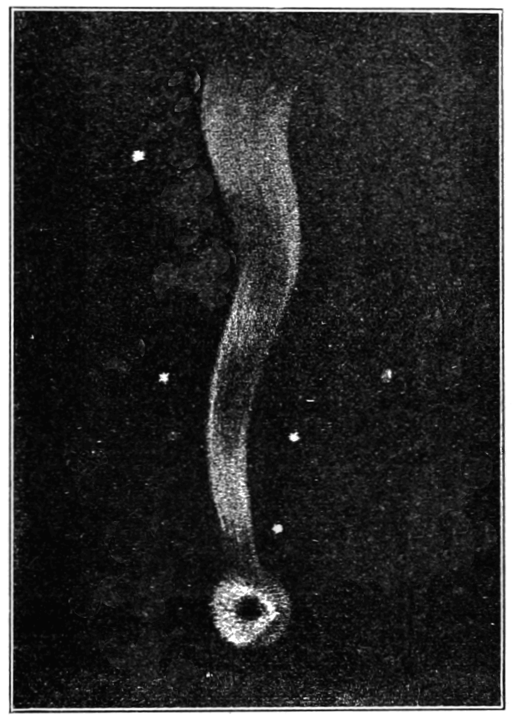
\includegraphics[width=.35\linewidth]{cometa}
\caption{Registro da passagem do cometa Halley em 1682}
\end{figure}

\begin{enumerate}
\item 1) Uma pessoa que nasceu em 2020 vai ter a oportunidade de avistar o cometa Halley pela primeira vez em que ano? E uma que venha a nascer no ano 2200? E no ano 3000?

\item Qual foi o ano em que o cometa Halley pode ter sido avistado pela primeira vez para uma pessoa que nasceu em 1900? E uma que nasceu em 1500?

\item Em uma folha de papel à parte, descreva como obter a resposta para questões como as anteriores para um amigo fictício que tenha terminado o Ensino Médio, mas não tenha resolvido essas questões. Tenha em mente que o objetivo não é explicar como resolver o problema, mas descrever um procedimento que permita ao seu colega obter respostas. Use texto, expressões matemáticas, esquemas visuais ou outros recursos que possam ajudar a deixar as suas instruções o mais claras possível.

\item Troque as instruções com um colega, e seguindo os passos que ele descreveu, obtenha o ano do primeiro possível avistamento do cometa Halley para alguém que tenha nascido nos anos: 2500, 1000 e 2290.

\item Antes de devolver a resolução para o seu colega, avalie-a considerando os seguintes aspectos: Ele seguiu a mesma estratégia que você? Na sua opinião, qual dos dois conjuntos de instruções é mais fácil de seguir e porquê?
\end{enumerate}

\end{task}



\arrange{Boas instruções}
\label{comp-arr1}

As atividades anteriores mostraram que não é simples criar um conjunto de instruções que resolve um determinado problema de modo que uma pessoa seja capaz de compreendê-las e segui-las sem poder fazer mais perguntas ou pedir esclarecimentos. Por isso é importante que fique claro tanto o significado de cada instrução, quanto a ordem em que elas devem ser executadas.

No caso de criarmos instruções para um computador seguir (um conjunto finito de instruções com fluxo bem definido também pode ser chamado de algoritmo), essa exigência fica ainda maior, pois o computador não consegue usar um pouco de bom senso ou conhecimentos adicionais sobre a situação para complementar as instruções ou tomar decisões, caso isso seja necessário. Para um computador, todas as instruções devem ser dadas de modo que ele seja capaz de executar e o fluxo das instruções deve estar absolutamente claro na descrição.

\explore{A representação via fluxogramas}
\label{comp-exp2}
\clearmargin
\begin{objectives}{Fluxogramas}
{
\begin{itemize}
\item Compreender como sistematizar soluções algorítmicas fazendo uso de recursos como a linguagem matemática, fluxogramas ou linguagens de programação.
\end{itemize}
}{1}{2}
\end{objectives}
\begin{sugestions}{Fluxogramas}
{
\textbf{Organização da turma}: esta atividade pode ser resolvida individualmente.

\textbf{Dificuldades previstas}: de acordo com a BNCC, os estudantes já devem ter interagido com fluxogramas no Ensino Fundamental e como os fluxogramas que propomos são simples, não devem apresentar desafios. O formato e a cor das partes dos fluxogramas segue um padrão internacional, mas isso não é importante para os usos que faremos neste módulo.

\textbf{Linguagem}: o significado do sinal de igual em linguagens de programação é diferente do significado usual em matemática. Ele deve ser entendido como a ação "atribua à variável na esquerda o valor especificado na direita". Vide discussão na próxima seção.

\textbf{Duração}: 30 minutos, completando uma aula com a discussão do Organizando a seguir.
}{1}{2}
\end{sugestions}
\begin{answer}{Fluxogramas}
{
\begin{enumerate}
\item 
\begin{enumerate}
\item R\$ $120{,}00$ e R\$ $285<00$, 
\item 2366.
\end{enumerate}

\item Um fluxograma que representa uma solução que usa um processo repetitivo até encontrar o ano de passagem do cometa é apresentado na imagem da próxima seção.
\end{enumerate}
}{1}
\end{answer}

Ao longo deste módulo, vamos conhecer várias ferramentas que nos permitam criar instruções que possam ser realizadas por um computador. Afinal, estamos procurando desenvolver habilidades e ferramentas que nos permitam criar algoritmos, e algoritmos podem ser usados para criar programas e aplicativos que realizem certas tarefas para nós!

Uma dessas ferramentas é o \textbf{fluxograma}. Trata-se de uma forma de representar visualmente a maneira como as instruções (ou comandos) se relacionam e qual a ordem em que devem ser realizadas (ou executados).

Você já deve ter visto esquemas visuais como o mostrado abaixo, que esquematiza o processo, de decisão nesse caso, sobre a pertinência de compartilhar uma notícia.

\begin{figure}[H]
\centering

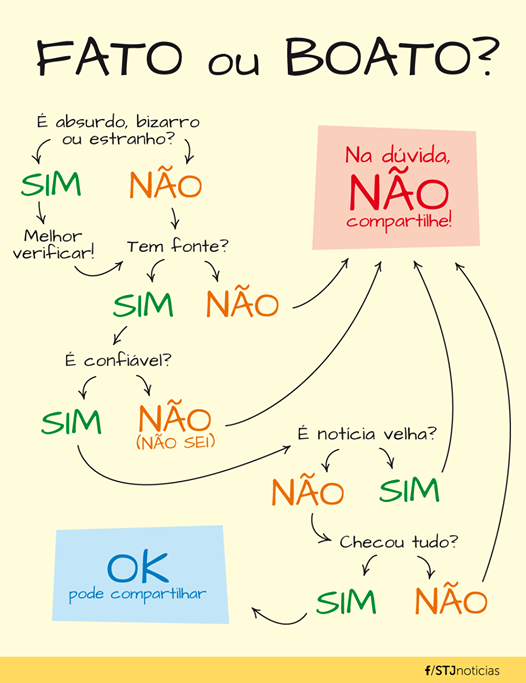
\includegraphics[width=.5\linewidth]{fluxograma_fake}
\caption{campanha do Superior Tribunal de Justiça}
\label{}
\end{figure}

Neste módulo, faremos um uso mais específico e rigoroso desse recurso, mas a intenção é a mesma da imagem acima: representar visualmente um processo com múltiplas etapas e ações.

\clearpage
\begin{task}{Fluxogramas}
\label{comp-task3}

A imagem a seguir mostra dois fluxogramas que resolvem as atividades anteriores. Leia-os com atenção e, se necessário, volte às atividades \hyperref[comp-task1]{1} e \hyperref[comp-task2]{2} para relembrar.

\begin{figure}[H]
\centering

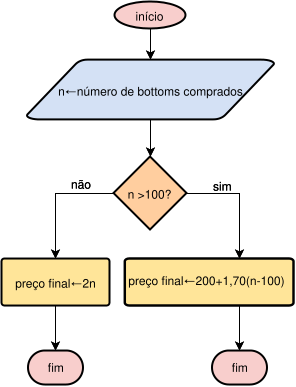
\includegraphics[width=.45\linewidth]{Figuras/fluxograma1}
\hspace{1em}
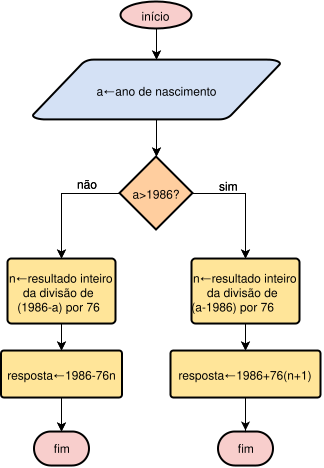
\includegraphics[width=.45\linewidth]{Figuras/fluxograma2}
\end{figure}

\begin{enumerate}
\item Utilize os fluxogramas para resolver os problemas das atividades \hyperref[comp-task1]{1} e \hyperref[comp-task2]{2} para os seguintes casos:

\begin{enumerate}
\item Qual seria o valor da compra para 60 bottons? E para 150?

\item Em que ano o cometa Halley poderá ser avistado pela primeira vez por alguém que tenha nascido no ano de 2300?
\end{enumerate}

\item Descreva a sua solução para a \hyperref[comp-task2]{Atividade 2} na forma de um fluxograma.
\end{enumerate}

\end{task}

\begin{reflection}
O que você achou dos fluxogramas como forma de apresentar um conjunto de instruções?
\end{reflection}

\arrange{Fluxogramas}
\label{comp-arr2}

Os fluxogramas são uma maneira de representar algoritmos que fazem uso de um arranjo visual para deixar claro o fluxo de comandos. Embora seja conveniente em muitas situações, eles não são recomendados para algoritmos muito complexos ou longos. Uma outra limitação dos fluxogramas é que eles não podem ser interpretados diretamente por um computador.

Mesmo assim, eles ainda podem ser uma forma rápida para organizar o seu raciocínio quando estiver pensando em um algoritmo. Por isso, consideramos que vale a pena mostrar mais um exemplo que ilustra uma situação não mostrada anteriormente: um processo repetitivo.

Considere a seguinte solução (descrita na forma textual) para a \hyperref[comp-task2]{Atividade 2}:

Se o ano de nascimento for maior que 1986, então some 76 a 1986 até que o resultado seja maior ou igual ao ano de nascimento. Quando isso ocorrer, o resultado da última soma é a resposta.
Se o ano de nascimento for menor do que 1986, então subtraia 76 a 1986 até que o resultado seja menor que ano de nascimento. Quando isso ocorrer, some 76 ao resultado da última soma e essa será a resposta.

Como fluxograma, ela pode ser representada como mostrado a seguir.

\begin{figure}[H]
\centering

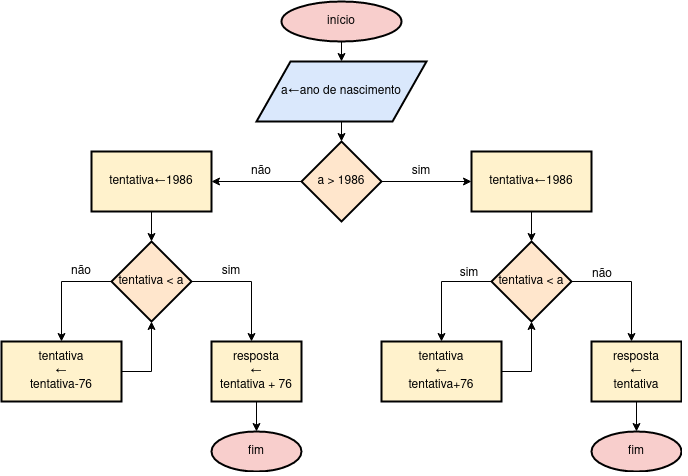
\includegraphics[width=\linewidth]{fluxograma3}
\end{figure}

Três coisas merecem atenção neste fluxograma.
Primeiro, a variável tentativa, que não apareceu nos fluxogramas anteriores. Ela é usada para armazenar em qual ano estamos à medida que somamos ou subtraímos 76 até encontrar a resposta. Na descrição verbal não é necessário mencioná-la, mas em uma linguagem de programação precisamos armazenar todos os resultados que desejamos usar posteriormente em alguma variável. Em um fluxograma também poderíamos evitar o seu uso, se escrevêssemos algo como "some 76 ao ano", mas a prática de armanzenar o resultado em uma variável é boa para não deixar dúvidas nas instruções seguintes.

Segundo, a ocorrência de ciclos: esses ciclos representam processos repetitivos, ou iterativos. Focando no que está mais à esquerda, ele diz o seguinte: cheque se a tentativa é menor do que a, se não for, subtraia 76 e volte para a checagem. Isso faz com que o algoritmo repita essa subtração até que o resultado encontrado seja menor do que a. No ciclo do lado direito, ocorre o mesmo mas com adições (veja que o lado direito do fluxograma é acionado quando a é maior do que 1986).

O terceiro aspecto que merece atenção são os comandos que são realizados dentro dos ciclos. Vamos focar novamente no que está mais à esquerda: tentativa = tentativa + 76. Note que essa expressão, do ponto de vista matemático, representa uma equação sem solução. Mas em grande parte das linguagens de programação, o sinal de igual significa "guarde o resultado da direita na variável à esquerda". Nesse caso, o computador primeiro calcula o valor do lado direito (somando 76 ao valor atual da variável tentativa) e então guarda na mesma variável (tentativa) o resultado (perdendo o valor anterior, o que não é um problema, pois já testamos e o descartamos).

\begin{observation}{}
É importante ter muito cuidado com expressões como "\verb|t=t+76|". Em um contexto matemático, o sinal de igual nessa expressão significa uma equivalência entre os valores do seu lado direito e esquerdo. Nesse caso específico, a expressão é uma equação sem solução (pois não existe valor de t que satisfaça a igualdade proposta).

Em linguagens de programação, o sinal de igual é normalmente usado para designar uma atribuição: a variável à esquerda do sinal deve receber o valor à direita. Inclusive, nesse contexto, a expressão \verb|t+76=t| é totalmente diferente de \verb|t=t+76| (na verdade, a primeira expressão está incorreta pois o conteúdo à esquerda do sinal de igual não é uma variável). Em algumas linguagens, a atribuição não é feita com o símbolo \verb|=|, mas com \verb|:=| ou \verb|<-| (imitando a seta $\leftarrow$).

Esse uso computacional do símbolo = deve ser evitado fora do contexto de algoritmos, pois provavelmente será interpretado em termos matemáticos.
\end{observation}

Processos repetitivos são muito comuns em algoritmos e voltaremos a eles em breve.

\know{Instruções para um computador}
\label{comp-know1}

Para que um computador seja capaz de seguir instruções que realizem alguma tarefa, é necessário que o algoritmo seja escrito em uma linguagem de programação. Uma linguagem de programação nada mais é do que uma maneira muito estruturada de descrever um algoritmo. A necessidade de clareza e estrutura para que um computador consiga interpretar um algoritmo faz com que certos elementos aparentemente estranhos sejam usados para organizar o fluxo das instruções.

\begin{knowledge}
Existem centenas de linguagens de programação em uso na atualidade, cada uma com certas vantagens e desvantagens e com diferentes níveis de popularidade. Atualmente, Python é uma linguagem muito utilizada em vários contextos e conta com muitos materiais para autoestudo na internet. Javascript é um outro exemplo, mas seu uso é mais comum em páginas de internet. A linguagem C é muito usada, mas normalmente para programas mais técnicos que precisem de alto rendimento.
\end{knowledge}

A imagem abaixo mostra dois algoritmos escritos em uma linguagem de programação chamada \textbf{Portugol}, que tem seus comandos em português. Apesar de não ser usada comercialmente, essa é a linguagem que sugerimos para você neste capítulo.

As instruções descritas abaixo em Portugol são as mesmas descritas anteriormente com fluxogramas. Leia com calma e tente compreender como as duas representações se relacionam.

\begin{figure}[H]
\centering

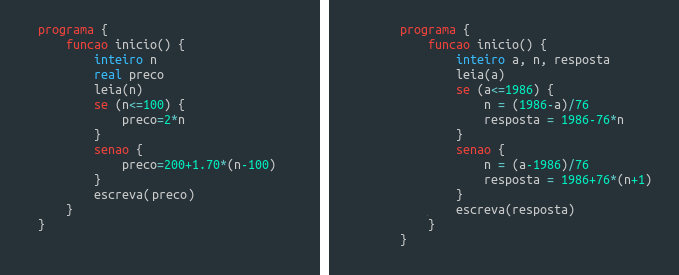
\includegraphics[width=\linewidth]{algoritmos1}
\end{figure}

Você pode acessar um ambiente online que permite a execução destes algoritmos em \url{portugol-webstudio.cubos.io}. Caso você não esteja familiarizado com esse tipo de recurso, sugerimos o vídeo \url{youtu.be/6OIADpFImtc} como ponto de partida.

\explore{Algoritmos para problemas matemáticos}
\label{comp_exp3}
\begin{texto}
{
As duas atividades propostas nesta seção focam no uso de variáveis e operações aritméticas entre elas.

A intenção do Organizando que encerra esta seção é salientar uma característica de linguagens de programação: a limitação dos comandos disponíveis. Na verdade, essa é uma limitação que não vale apenas para linguagens de programação, mas para qualquer software. Conhecer as limitações e como elas podem ser contornadas nos torna usuários mais hábeis. No caso específico desta seção, a limitação refere-se ao fato de Portugol não possuir um comando "arredonde para cima", portanto, isso precisa ser implementado a partir de outros comandos disponíveis na linguagem (combinando o cálculo do resto de uma divisão inteira com um condicional).

O que importa aqui é a consciência da limitação e não o domínio sobre como implementar o arredondamento para cima em uma linguagem de programação. Além disso, essa discussão traz de volta o conceito de condicional (o comando "se"{} do algoritmo mostrado) que será o foco da próxima seção.
}
\end{texto}
\marginpar{\vspace{-1em}}
\begin{objectives}{Contêineres}
{
\begin{itemize}
\item Compreender como sistematizar soluções algorítmicas através de recursos como a linguagem matemática, fluxogramas ou linguagens de programação.

\item Compreender os conceitos básicos de uma linguagem de programação: variáveis
\end{itemize}
}{1}{1}
\end{objectives}
\marginpar{\vspace{-2.5em}}
\begin{sugestions}{Contêineres}
{
\textbf{Organização da turma}: sugerimos a resolução desta e da próxima atividade conjuntamente e, especialmente por causa da segunda atividade, recomendamos a organização da turma em duplas.

\textbf{Duração}: essa e a próxima atividade juntas devem ocupar em torno de 1 aula.

\textbf{Comentários para o laboratório}: a implementação da solução a este problema em Portugol é muito próxima ao que os estudantes devem descrever aqui, pois ao fazermos a divisão entre dois números inteiros e armazenarmos em uma variável inteira, o Portugol armazena o quociente da divisão inteira (com resto), causando o efeito de arredondar para baixo.

\textbf{Conexões}: você pode discutir o conceito de volume de paralelepípedos e relembrar o significado da divisão em termos de medida.
}{1}{1}
\end{sugestions}
\marginpar{\vspace{-1em}}
\begin{answer}{Contêineres}
{
\begin{enumerate}
\item $3750$

\item $588$

\item Calculamos a quantidade de conteineres que cabem em cada uma das dimensões: $n1=X/ A$, $n2=Y\slash B$ e $n3=25\slash C$, sempre considerando a parte inteira do quociente. O total de conteineres que podem ser levados será: total = $n1\times n2\times n3$.
\end{enumerate}
}{0}
\end{answer}
\begin{objectives}{Um professor em cada van}
{
\begin{itemize}
\item Compreender como sistematizar soluções algorítmicas através de recursos como a linguagem matemática, fluxogramas ou linguagens de programação.

\item Compreender os conceitos básicos de uma linguagem de programação: variáveis.
\end{itemize}
}{1}{2}
\end{objectives}
\begin{sugestions}{Um professor em cada van}
{
\textbf{Organização da turma}: em duplas.

\textbf{Duração}: essa atividade e a anterior devem ocupar em torno de 1 aula.

\textbf{Dificuldades previstas}: a interpretação do enunciado da questão pode gerar algumas dúvidas, por isso dê tempo para que os alunos compreendam matematicamente o problema antes de partir para os itens de natureza computacional.

\textbf{Comentários para o laboratório}: a implementação desta solução é um pouco mais desafiadora do que a descrição verbal por causa do procedimento de "arredondar para cima", que não é oferecido de forma direta em Portugol. Na resolução da atividade essa dificuldade não deve emergir, mas ela será aprodundada na seção organizando logo a seguir.
}{1}{2}
\end{sugestions}
\begin{answer}{Um professor em cada van}
{
\begin{enumerate}
\item $16{,}5$

\item Calcule $n$ dividido por $13$ e arredonde o resultado para cima se houver parte decimal

\item Sim, Não

\item Calcule n dividido por $13$ e arredonde o resultado para cima se houver parte decimal. Esse resultado, vamos chamar de $p$, é igual ao número de vans necessárias e igual ao número mínimo de professores. O número máximo de professores, chamemos de $\max$, é dado por $\max=14p-n$
\end{enumerate}
}{1}
\end{answer}

Dois recursos são muito comuns na criação de algoritmos, não importando se descrevemos na forma textual, com fluxograma ou em uma linguagem de programação: condicionais e repetições. Além desses dois recursos, o conceito de variável é especialmente importante quando pensamos em linguagens de programação, seja ela qual for.

Já conhecemos esses três elementos nas atividades anteriores e nas atividades a seguir vamos ter a chance de explorá-los com mais profundidade.

\begin{task}{Contêineres}
\label{comp-task4}
O transporte em grandes navios de carga se dá através de contêineres, que são caixas metálicas grandes, dentro das quais as empresas acomodam seus produtos da maneira que desejar. Porém, a maneira como os contêineres são colocados nos navios costuma ser determinada pelo sistema de carregamento disponível nos portos. Imagine um porto que, por restrição nos equipamentos disponíveis, carregue seus contêineres todos alinhados, na mesma direção e com os lados paralelos aos lados da área de carregamento do navio, como mostrado na figura abaixo.

\begin{figure}[H]
\centering

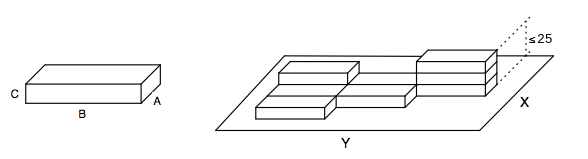
\includegraphics[width=.7\linewidth]{conteineres}
\end{figure}

A administradora desse porto está com problemas para determinar quantos contêineres de dimensões $A$, $B$ e $C$ (em metros) podem ser colocados em um navio que tenha área de carregamento nas dimensões $X$ e $Y$ (em metros). Observe que a dimensão $A$ dos contêineres deve ser carregada paralelamente à dimensão $X$ dos contêineres, o mesmo ocorre para as dimensões $B$ e $Y$.

Além dessas restrições, há uma limitação de altura imposta pelas autoridades portuárias que diz que a pilha de contêineres não pode ultrapassar $25$ metros de altura.

\begin{enumerate}
\item Quantos contêineres de dimensão (em metros) $A=3$, $B=4$, $C=1$ cabem em um navio com área de carregamento com dimensões $X=30$ e $Y=60$?

\item Quantos contêineres de dimensão (em metros) $A=4$, $B=8$, $C=2$ cabem em um navio com área de carregamento com dimensões $X=30$ e $Y=60$?

\item Descreva, com suas palavras, como determinar quantos contêineres de dimensões $A$, $B$ e $C$ cabem em um navio com espaço de carregamento igual a $X$ e $Y$.
\end{enumerate}
\end{task}

\begin{task}{Um professor em cada van}
\label{comp-task5}

Uma escola costuma organizar passeios com frequência e para levar os alunos conta com vários motoristas de vans. Essas vans possuem $14$ lugares, além do assento do motorista. Por questão de segurança, a direção da escola exige que sempre haja um professor em cada van, não importando o número de alunos. Felizmente, a escola tem contato com muitos motoristas de vans.

\begin{enumerate}
\item Quantos professores serão necessários para acompanhar os estudantes em um passeio em que $200$ estudantes desejem participar? E em um passeio em que $65$ estudantes desejem participar?

\item Descreva com suas palavras, e de forma clara, como obter a quantidade mínima de professores necessários para acompanhar um passeio em que $n$ estudantes estejam interessados em participar.

Em algumas ocasiões, porém, há mais professores dispostos a acompanhar os estudantes do que o necessário. Em geral, a direção gosta dessa situação pois cada professor fica responsável por menos estudantes. Porém, já aconteceu de não haverem lugares disponíves nas vans para os professores adicionais, e a escola não pretende contratar vans adicionais.

\item Se houverem $200$ estudantes interessados e $20$ professores disponíveis, haverá lugar para todos os professores nas vans sem que seja necessário contratar vans adicionais? E se forem $75$ estudantes e $10$ professores?

\item Descreva com suas palavras e de forma clara como descobrir o número máximo de professores que podem acompanhar $n$ estudantes em um passeio sem que seja necessário contratar mais vans.
\end{enumerate}

\end{task}

\arrange{O computador sabe menos do que você}
\label{comp-arr3}

Para resolver as duas atividades anteriores você deve ter utilizado apenas algumas operações: soma, subtração, multiplicação, divisão e arredondamentos. As quatro primeiras estão diretamente disponíveis em qualquer linguagem de programação, mas a quinta delas nem sempre. Vamos discuti-la em mais detalhes.

Na atividade Um professor em cada van você deve ter utilizado o recurso de arredondar para cima para descobrir o número mínimo de professores necessários para acompanhar a turma. Por exemplo, se $30$ alunos quiserem participar de uma viagem, calculamos . Logo, precisamos de mais de $2$ professores, ou seja, $3$. Matematicamente, dizemos que obtivemos o menor número inteiro maior ou igual ao resultado da divisão. Informalmente, dizemos que estamos "arredondando para cima". Porém, o Portugol (e outras linguagens de programação) não entende o comando "arredonde para cima"{} ou "obtenha o menor número inteiro maior ou igual". Então, como poderíamos descrever para o computador esse processo?

Para fazer isso, podemos utilizar duas operações que a maioria das linguagens de programação oferece: quociente da divisão (representada por "\verb|/|") e resto da divisão entre dois números inteiros (representada por "\verb|%|"). A operação \verb|%| só pode ser realizada entre dois números inteiros e também retorna como resultado um número inteiro. Já a operação \verb|/| retorna um número real como quociente se os valores envolvidos forem números reais e a parte inteira do quociente se os números envolvidos forem inteiros. Por exemplo, \verb|9/4| terá como resultado $2$, \verb|9%4| terá como resultado $1$ e \verb|7.2/4.8| terá como resultado $1.5$.

No caso do problema posto na atividade, devemos adicionar uma van se a divisão do número de interessados por 13 tiver resto maior do que zero. Em Portugol, uma possibilidade seria essa:

\begin{figure}[H]
\centering

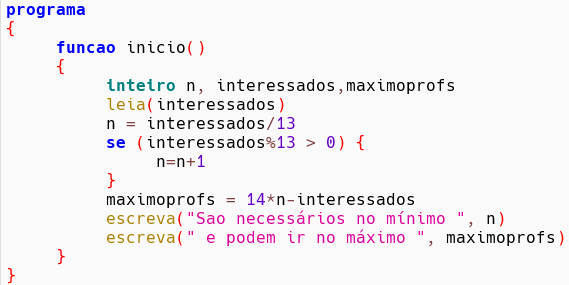
\includegraphics[width=.7\linewidth]{algoritmos2}
\end{figure}

Veja que esse algoritmo primeiro considera que o número mínimo de professores é igual ao resultado inteiro (veja que a variável n é do tipo inteiro) da divisão do número de interessados por $13$. Depois, se o resto da divisão por $13$ for maior do que zero, o algoritmo soma $1$ ao número mínimo de professores.

\explore{Condicionais}
\label{comp-exp4}
\begin{texto}
{
Esta seção foca no uso de estruturas condicionais. Apesar de já terem aparecido nas seções anteriores, a atividade a seguir propõe uma situação em que é necessário utilizar condicionais de forma mais sofisticada do que nas anteriores. A sofisticação não vem da dificuldade matemática da questão, mas pela atenção necessária para que as instruções fiquem claras.

A intenção do Organizando desta seção é refletir um pouco sobre algoritmos com fluxos mais complexos devido ao uso de condições encadeadas. Isso é muito comum em algoritmos e por isso é importante compreender como interpretá-los.

Um exemplo simples e interessante que pode ser usado tanto para avaliar o trabalho desenvolvido nesta seção quanto para estender a discussão é o algoritmo para determinar se uma pessoa é maior de idade a partir do dia, mês e ano de seu nascimento e da data de hoje. Note que se a diferença entre os anos for maior do que 18 não é necessário sequer checar o mês. Também não é necessário checar o dia do nascimento se o mês do 18° aniversário já passou. Construir e discutir o fluxograma deste algoritmo pode ser bastante rico.	
}
\end{texto}
\clearmargin
\begin{objectives}{Cubos conectados}
{
\begin{itemize}
\item Compreender como sistematizar soluções algorítmicas através de recursos como a linguagem matemática, fluxogramas ou linguagens de programação.

\item Compreender os conceitos básicos de uma linguagem de programação: condicional.
\end{itemize}
}{1}{2}
\end{objectives}
\begin{sugestions}{Cubos conectados}
{
\textbf{Organização da turma}: sugerimos que os estudantes resolvam essa atividade em grupo, pois ela exige não apenas a compreensão da situação proposta como também atenção aos detalhes na elaboração da solução da questão 5 e esmero na apresentação dessa solução.

\textbf{Duração}: 1 aula.

\textbf{Sugestões gerais}: o professor pode transformar essa atividade em um mini-projeto em que os grupos deverão apresentar para a turma toda as suas soluções para a questão. Nesse caso, sugerimos o uso de uma cartolina e cores para registro da resolução. Outra possibilidade, é trocar as soluções entre os grupos para que eles avaliem a clareza das soluções dos colegas.

\textbf{Dificuldades}: é comum os estudantes não representarem ou descrevem a relação entre as diferentes condições de maneira adequada. Os condicionais que resolvem este problema podem estar um dentro do outro ou um depois do outro, e o fluxo entre os comandos são diferentes nesses casos, como será discutido na seção Organizando a seguir.

\textbf{Conexões}: o início da atividade toca no tópico volume de paralelepípedos e unidades de medida de comprimento e volume de forma bastante simples. Esta pode ser uma boa oportunidade para uma revisão breve antes que os estudantes se engajem com as questões da atividade.
}{1}{2}
\end{sugestions}
\begin{answer}{Cubos conectados}
{
\begin{enumerate}
\item $500$ litros, $400$ litros, $0$ litros

\item $500$ litros, $500$ litros, $250$ litros

\item $600$ litros, $600$ litros, $600$ litros
\end{enumerate}
}{1}
\end{answer}
\begin{answer}{Cubos conectados}
{
\begin{enumerate}
\item $800$ litros, $800$ litros, $800$ litros

\item Existem muitas maneiras de resolver esse problema. Duas delas são discutidas na seção Organizando a seguir. Sugerimos que as soluções dadas pelos estudantes sejam comparadas levando em conta as discussões propostas a seguir.
\end{enumerate}
}{1}
\end{answer}

As sentenças que fazem uso do condicional (aqui chamadas simplesmente de condicionais) são um componente central em qualquer linguagem de programação e, na verdade, em boa parte dos recursos computacionais que utilizamos explícita ou implicitamente.

No caso das planilhas eletrônicas, por exemplo, elas podem ser usadas para que uma célula mostre um conteúdo que depende do conteúdo de uma outra célula. Um exemplo simples é mostrado abaixo. Imagine que um professor tenha uma planilha onde registra as notas dos seus estudantes em duas provas. Além de calcular a média das duas notas, ele deseja que a planilha mostre se cada estudante está, ou não, de recuperação de acordo com o seguinte critério: se a média for menor do que $6$ então o estudante está de recuperação, senão está aprovado.

\begin{figure}[H]
\centering

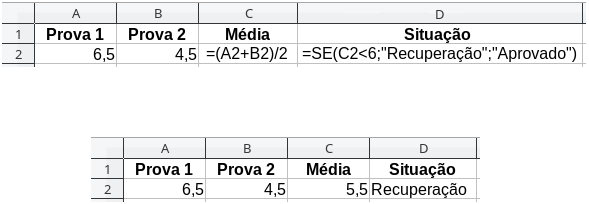
\includegraphics[width=.7\linewidth]{planilha}
\end{figure}

Note que o comando descrito na frase "se a média for menor do que 6, então o estudante está de recuperação, senão está aprovado"{} é composto por três partes: uma condição $(C2<6)$, o que deve ser feito se a condição for verdadeira (escrever a palavra "Recuperação"{} na célula) e o que deve ser feito se a condição for falsa (escrever "Aprovado"{} na célula). Isso está condensado no conteúdo da célula $D2$ mostrada acima.

Nas atividades anteriores, usamos o mesmo raciocínio para resolver o problema do cometa Halley (se o ano de nascimento fosse maior do que 1986 a resolução seguia por um caminho, se fosse menor seguia por outro) e o problema sobre o número de professores (se houvesse resto na divisão, era necessário contratar mais uma van). Quando representamos um algoritmo na forma de um fluxograma, condicionais são representadas como bifurcações no fluxo das instruções, de modo que um ou outro lado deve ser seguido conforme a condição estipulada.

\begin{figure}[H]
\centering

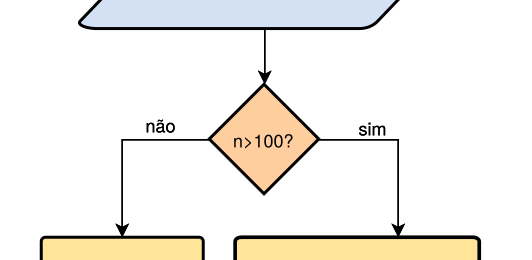
\includegraphics[width=.7\linewidth]{figura_p1_01}
\end{figure}

A próxima atividade vai exigir um uso mais sofisticado de condicionais do que as atividades que resolvemos até agora.

\begin{task}{Cubos conectados}
\label{comp-task6}

Uma empresa que produz detergente transporta o produto bruto em cubos metálicos com lados iguais a $1$ metro. Para facilitar o enchimento destes cubos, eles possuem uma abertura pequena, como mostrado na figura abaixo, que permite conectar dois cubos durante o enchimento. Assim, à medida que o líquido é despejado, ao atingir a altura da abertura, o líquido começa a escoar para o segundo cubo. Se houver líquido suficiente, o terceiro cubo também poderá receber uma parte.

Por questões de logística, a empresa atualmente enche sempre $3$ cubos conectados por essas aberturas, e isso é feito despejando-se o líquido sempre a partir da tampa do cubo mais à esquerda, como mostrado na vista lateral abaixo.

\begin{figure}[H]
\centering

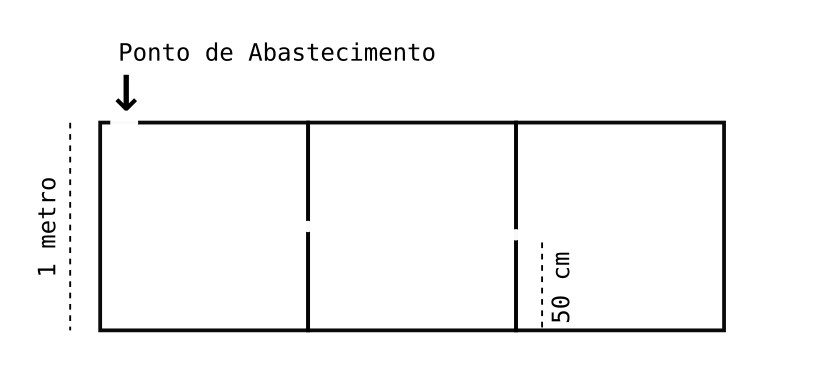
\includegraphics[width=.8\linewidth]{cubos1}
\end{figure}

Por exemplo, se forem injetados $600$ litros de detergente, os cubos ficarão como mostrado a seguir, com $500$ litros no primeiro, $100$ litros no segundo e $0$ no terceiro.

\begin{figure}[H]
\centering

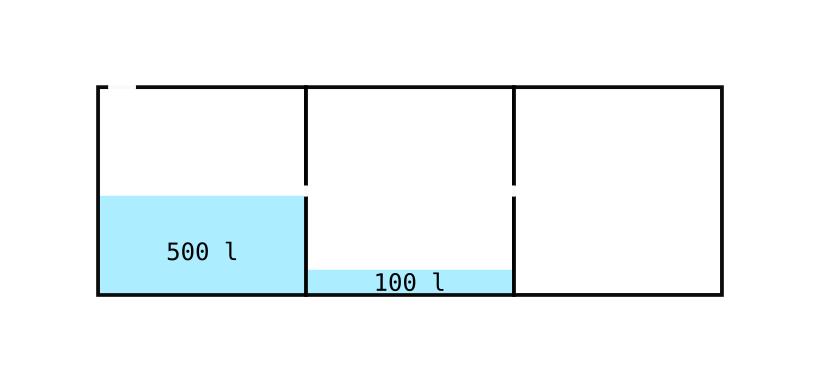
\includegraphics[width=.8\linewidth]{cubos2}
\end{figure}

\begin{enumerate}
\item Quantos litros haverá em cada cubo se forem injetados $900$ litros de detergente?

\item Quantos litros haverá em cada cubo se forem injetados $1250$ litros de detergente?

\item Quantos litros haverá em cada cubo se forem injetados $1800$ litros de detergente?

\item Quantos litros haverá em cada cubo se forem injetados $2400$ litros de detergente?

\item A empresa quer que você crie um algoritmo que permita saber qual é o volume de detergente em cada um dos três cubos quando uma quantidade $N$ (em litros) é despejada no conjunto. Apresente a sua solução de maneira esquemática, isto é, sem usar muito texto.
\end{enumerate}


\end{task}

\arrange{Combinando condições}
\label{comp-arr4}

Leia com atenção os dois fluxogramas abaixo. Ambos foram criados para determinar se um número dado é múltiplo de 6 a partir do seguinte resultado: um número é múltiplo de $6$ se for múltiplo de $2$ e de $3$.

\begin{figure}[H]
\centering

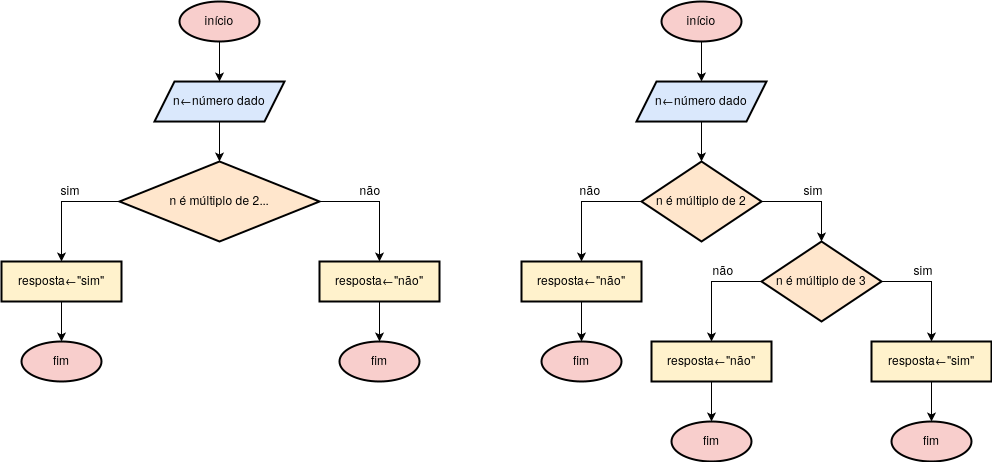
\includegraphics[width=\linewidth]{fluxograma4}
\end{figure}

\begin{reflection}
Os dois fluxogramas são visualmente diferentes, mas o que você pode dizer sobre os resultados que cada um deles produz para diferentes valores de N?
\end{reflection}

Veja que no fluxograma da esquerda, temos uma única condição e ela testa, de uma só vez, se N é múltiplo de 2 e se N é múltiplo de 3. No fluxograma da direita temos duas condições e a segunda está "dentro"{} da primeira, sendo acionada apenas se a primeira for verdadeira. Apesar de estruturalmente diferentes, ambas produzem os mesmos resultados para qualquer valor de N. Como ambas estão corretas, a escolha por uma ou outra solução deve ser feita por outros critérios, como a clareza para o leitor, os recursos disponíveis na linguagem de programação que você esteja usando ou até mesmo considerações sobre a eficiência de cada algoritmo em termos de velocidade de processamento computacional (mas essa discussão é muito mais avançada do que os nossos objetivos no momento).

Agora, vejamos dois exemplos de flouxogramas que resolvem a atividade Cubos Conectados corretamente e que são visualmente muito diferentes.

\clearmargin
\begin{texto}
{
	Em termos de execução, o fluxograma da esquerda é mais eficiente, pois nem sempre faz todas as comparações. Porém, a sua versão escrita em uma linguagem de programação fica visualmente mais difícil de compreender do que o fluxograma da direita.
}
\end{texto}

\begin{figure}[H]
\centering

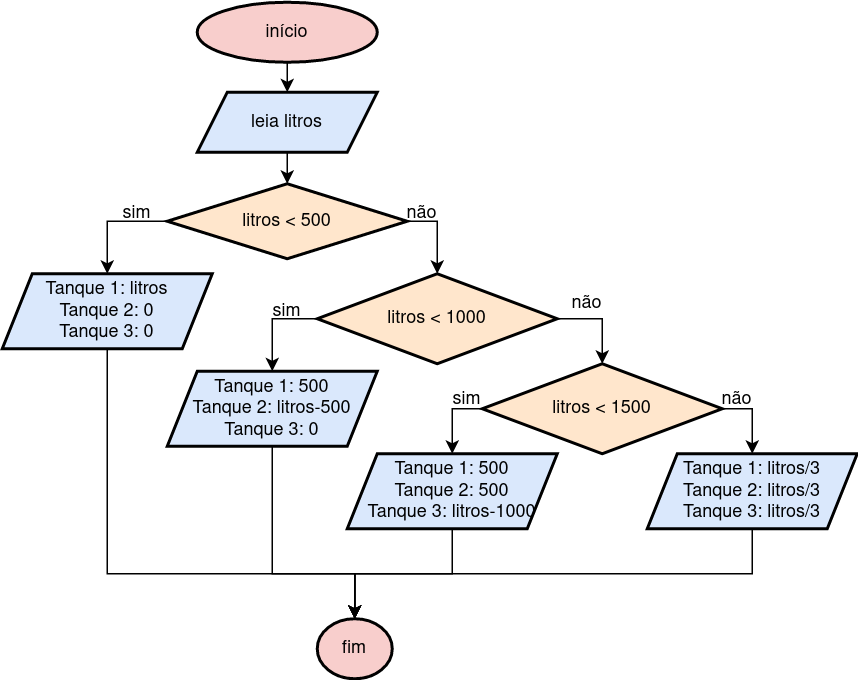
\includegraphics[height=.33\textheight]{fluxograma6}
\hspace{1em}
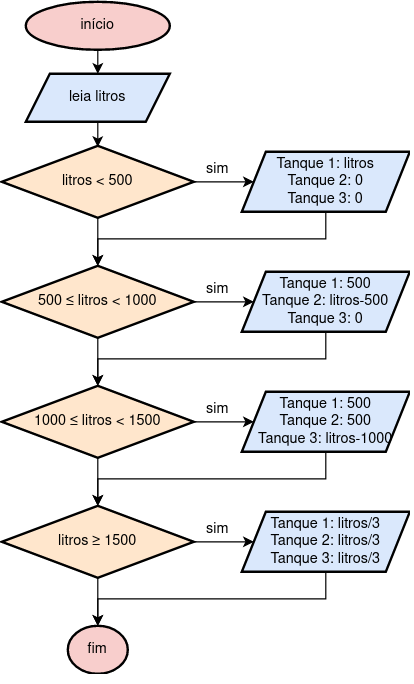
\includegraphics[height=.33\textheight]{fluxograma7}
\end{figure}

\begin{texto}
{
A seguir, mostramos os algoritmos em Portugol que implementam o que está representado acima nos dois fluxogramas.

\centering
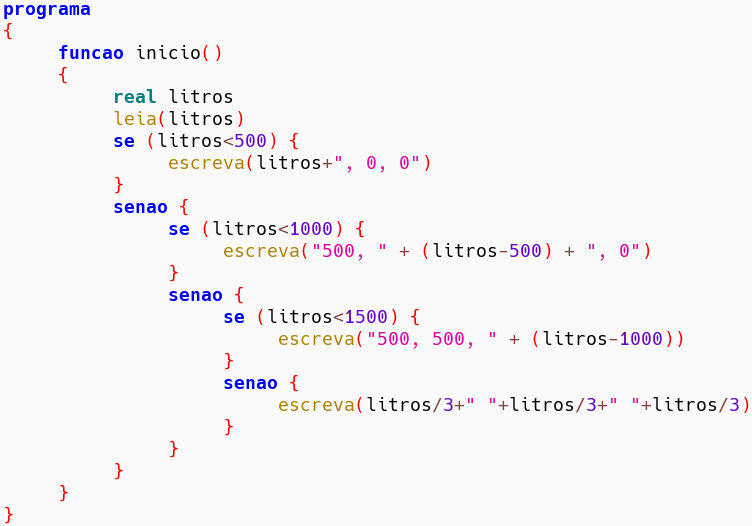
\includegraphics[width=.75\linewidth]{algoritmos13}

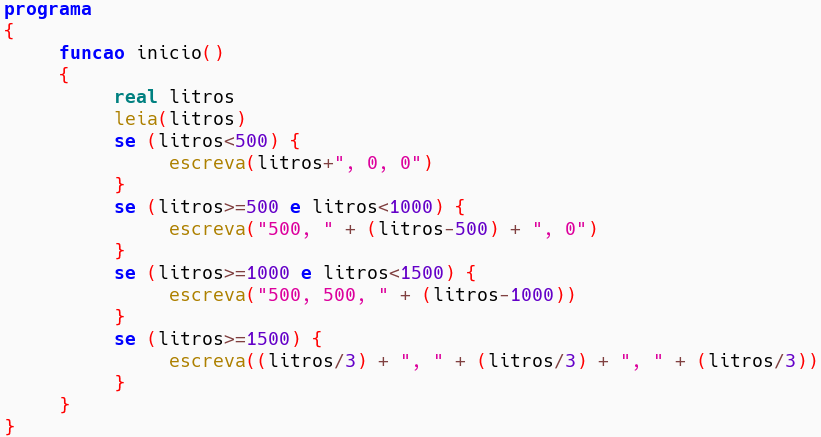
\includegraphics[width=.75\linewidth]{algoritmos12}
\justify

Outras soluções são possíveis. O importante é que os estudantes consigam seguir o fluxo de comandos do algoritmo, interpretando corretamente as condições e o que dever ser realizado à medida que cada uma delas é verdadeira ou falsa.
}
\end{texto}

Note que no fluxograma da esquerda, as condições estão encadeadas. Se o total de litros colocados for menor do que 500, o fluxo do algoritmo passa pelo bloquinho azul mas à esquerda e depois já vai para o fim, sem sequer considerar as demais condições.

No fluxograma da direita, as quatro condições são sempre analisadas, não importando se alguma delas já foi satisfeita e produziu a resposta corretamente.



\begin{reflection}
Você consegue pensar em algum argumento que permita concluir se um dos fluxogramas é melhor do que o outro?
\end{reflection}



\know{Condicionais}
\label{comp-know2}

Condições em linguagens de programação costumam ser escritas com o comando se, que você já viu anteriormente. O uso de várias condicionais em sequência, ou de uma dentro da outra, acompanhado ou não pelo comento senao, permite criar muitas variações para um mesmo algoritmo, como vimos com fluxogramas para a atividade dos Cubos Conectados.

Tente usar o comando se para escrever um algoritmo em Portugol que se comporte como cada um dos dois fluxogramas mostrados acima. E você não precisa parar por aí: é possível criar outras soluções corretas e diferentes para o problema. Que tal tentar?


\def\currentcolor{session1}
\begin{texto}
{
Esta seção é focada em estruturas de repetição, como o enquanto, que já usamos em problemas anteriores. O objetivo aqui é salientar o poder desse recurso para realizar tarefas que poderiam ser muito monótonas se feitas à mão.

Professor, faça a leitura e interpretação das duas representações discutidas no \textbf{Explorando} com seus estudantes, tendo certeza de que eles compreendem dois aspectos importantes em uma estrutura de repetição: a condição (m<10, nesse caso) e a delimitação dos comandos que são repetidos (delimitados pelas chaves em Portugol e pela sequência que parte da condição e volta para ela no fluxograma).

As duas atividades propostas abordam conteúdos com grande potencial do ponto de vista matemático: números primos e uma sequência numérica (chamada de sequência de Collatz) que envolve uma conjectura ainda em aberto.

A intenção do exemplo mostrado no \textbf{Organizando} é promover uma discussão, através de um algoritmo simples, sobre duas práticas comuns em estruturas de repetição: o uso de uma variável como contador e a passagem de valores entre variáveis.

A segunda atividade ele abre portas para muitos outros exemplos interessantes envolvendo sequências numéricas. Se seus estudantes estiverem com dificuldades, pode ser um bom momento para explorar sequências numéricas diversas e fixar alguns conceitos tratados até aqui. As sequências que são descritas via termo geral são mais simples do que as que são definidas via relação de recorrência. Alguns exemplos que são abordados em outros módulos do Livro Aberto são: Progressão Aritmética de primeira e segunda orgem, Progressão Geométrica, Números Triangulares e Números Hexagonais.
}
\end{texto}

\explore{Repetir e repetir}
\label{comp-exp5}

Repetir muitas vezes uma mesma ação é algo considerado cansativo para a maioria das pessoas. Porém, para muitas tarefas isso é necessário para se resolver algum problema ou atingir algum objetivo. Esse é um dos motivos que fazem dos computadores uma ferramenta tão útil: eles podem repetir comandos sem se cansar, sem perder a motivação ou a atenção e sem se distrair a ponto de cometerem erros. Historicamente, essa foi a motivação de diversos cientistas que, a partir do século 17, começaram a propor máquinas que fossem capazes de realizar cálculos aritméticos e que podem ser consideradas as avós dos computadores modernos.

\begin{knowledge}
As primeiras máquinas concebidas para realizar cálculos eram puramente mecânicas, ou seja, baseadas em engrenagens e encaixes físicos. Pesquise na internet pelas máquinas desenvolvidas pelos matemáticos Blaise Pascal e Gottfried Leibniz.
\end{knowledge}

\begin{texto}
{
	Note que da maneira como está escrito, o algoritmo não escreve o resultado da multiplicação por $10$, pois a condição da repetição é verdadeira até m ser igual a $9$.
}
\end{texto}
\clearmargin
\begin{objectives}{É primo ou não?}
{
\begin{itemize}
\item Compreender como sistematizar soluções algorítmicas através de recursos como a linguagem matemática, fluxogramas ou linguagens de programação.

\item Compreender os conceitos básicos de uma linguagem de programação: repetição.
\end{itemize}
}{1}{2}
\end{objectives}
\begin{sugestions}{É primo ou não?}
{
\textbf{Organização da turma}: sugerimos que essa atividade seja resolvida em conjunto, pela turma toda, uma vez que a etapa final (envolvendo a utilização do algoritmo criado) depende do uso de um computador ou celular e de um algoritmo completo e correto para o problema proposto.

\textbf{Duração}: 1 aula.

\textbf{Sugestões gerais}: os itens que podem ser identificados na discussão proposta no Para refletir são: 1) só é necessário verificar se um número  é divisor de um número  enquanto ; 2) a busca pode ser feita apenas até encontrarmos um divisor diferente de 1 e de ; e 3) só seria necessário checar se números primos são divisores, mas como não temos uma lista desses números disponível, essa propriedade não pode ser utilizada neste contexto.

\textbf{Conexões}: vários tópicos do Ensino Fundamental podem ser revisados ou discutidos em conexão com essa atividade. Entre eles, vale mencionar os conceitos de divisor e múltiplo, critérios de divisibilidade e o Crivo de Eratóstenes (que pode inclusive ser discutido sob o ponto de vista computacional também se os estudantes souberem usar variáveis do tipo vetor).
}{1}{2}
\end{sugestions}
\begin{answer}{É primo ou não?}
{
\begin{enumerate}
\item O objetivo das questões \titem{a)} e \titem{b)} é obter um algoritmo como o mostrado a seguir.

\begin{figure}[H]
\centering

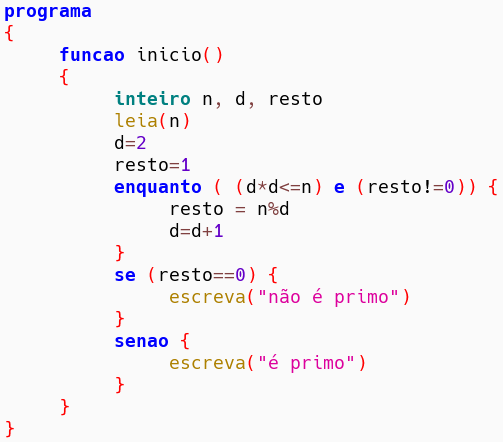
\includegraphics[width=.65\linewidth]{algoritmos3}
\end{figure}

\item Sim, é primo.

\item Se a turma notou a restrição de procurar divisores até , serão necessárias aproximadamente $2000$ verificações, ou seja, $2000$ segundos, que equivale a mais de meia hora. Se a turma tivesse uma lista de números primos, seria necessário apenas cerca de $300$ verificações, ou seja, $5$ minutos.
\end{enumerate}
}{0}
\end{answer}
\clearmargin

\begin{objectives}{A sequência de Collatz}
{
\begin{itemize}
\item Compreender como sistematizar soluções algorítmicas através de recursos como a linguagem matemática, fluxogramas ou linguagens de programação.

\item Compreender os conceitos básicos de uma linguagem de programação: repetição.
\end{itemize}
}{1}{1}
\end{objectives}
\marginpar{\vspace{-2.5em}}
\begin{sugestions}{A sequência de Collatz}
{
\textbf{Dificuldades}: este problema não deve oferecer muitas dificuldades do ponto de vista matemático. Do ponto de vista computacional, ele também é mais simples que a ativdiade anterior e essa escolha foi intencional, para servir como uma atividade de fixação.

\textbf{Organização da turma}: por ter objetivo maior de fixação e pela simplicidade matemática do problema, sugerimos que essa atividade seja resolvida individualmente ou em duplas, após uma discussão inicial com a turma toda para que se compreenda o pedido descrito no problema.

\textbf{Duração}: 1 aula.

\textbf{Para o laboratório}: com o algoritmo em mãos, várias explorações podem ser feitas, por exemplo: você consegue encontrar um valor para  que resulte em uma sequência de tamanho exatamente igual a 7? Qual é o número inteiro menor do que 50 que resulta na sequência com o maior número de termos?
}{1}{1}
\end{sugestions}
\marginpar{\vspace{-1em}}
\begin{answer}{A sequência de Collatz}
{
\begin{enumerate}
\item $6, 3, 10, 5, 16, 8, 4, 2, 1$
\item $52, 26, 13, 40, 20, 10, 5, 16, 8, 4, 2, 1$
\item \adjustbox{valign=t}
{
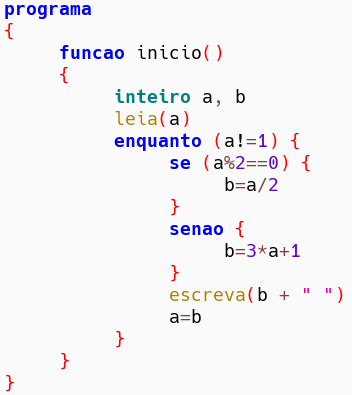
\includegraphics[width=.475\linewidth]{algoritmos4}
}
\end{enumerate}
}{1}
\end{answer}


Nas próximas atividades, vamos lidar com problemas que envolvem muitas repetições e que ainda são muito relevantes na atualidade. Para isso, observe como o ciclo apresentado no fluxograma abaixo é representado em Portugol.

\begin{figure}[H]
\centering

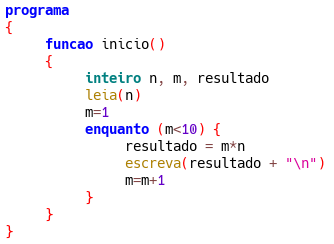
\includegraphics[width=.45\linewidth]{algoritmos5}
\hspace{1em}
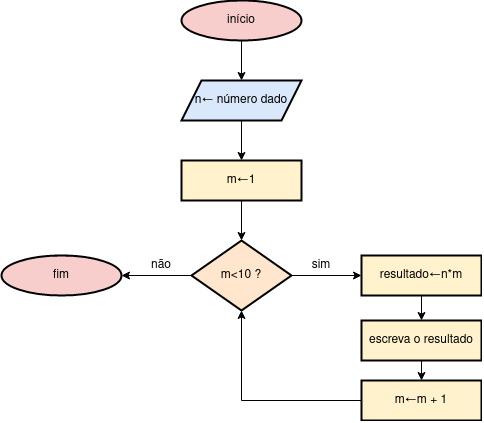
\includegraphics[width=.45\linewidth]{fluxograma5}
\end{figure}

Em Portugol, o ciclo é realizado pelo comando enquanto: quando o computador chega neste comando, ele entende que deve repetir os comandos dentro das chaves seguintes enquanto a condição colocada ($m<10$) for verdadeira. A cada repetição, a variável m tem o seu conteúdo aumentado em uma unidade, o que faz com que em algum momento o seu valor seja maior ou igual a $10$, violando a condição e fazendo com que a interpretação do algoritmo saia do ciclo.

Esse é um exemplo simples de uma estrutura de repetição, que poderia ser feita por uma pessoa sem grande esforço. Mas ela transmite muito bem a ideia de repetir alguma ação enquanto uma condição for verdadeira. Nas atividades a seguir, vamos propor algumas tarefas repetitivas que são muito trabalhosas quando feitas manualmente, por isso é ainda mais relevante utilizar um computador para fazê-las.

\begin{task}{É primo ou não?}
Você deve se lembrar que um número é chamado de primo se tiver exatamente dois divisores inteiros positivos diferentes: $1$ e ele mesmo. Por exemplo, o número $9$ não é primo, pois seus divisores são $1$, $3$ e $9$. Já o número $13$ é primo. O número 1 não é primo por que possui um único divisor inteiro positivo.

Até hoje, não existem métodos realmente rápidos para identificar se um número é primo ou não. Basicamente, todos os métodos existentes baseiam-se em testar se o número dado deixa resto zero quando é dividido pelos números menores do que ele. Imagina a quantidade de repetições necessárias para verificar se o número $4.000.037$ é primo!

\begin{enumerate}
\item Crie um algoritmo que verifica se um número é primo ou não.

\item Em conjunto com toda a turma escrevam um dos algoritmos criados na questão $1$ em Portugol.

\item Utilize esse algoritmo para verificar se o número $4.000.037$ é primo.

Você deve ter notado que o algoritmo responde quase que imediatamente se o número dado é primo ou não, mesmo sendo um número grande.

\item Se você conseguisse verificar um divisor a cada $1$ segundo, estime aproximadamente quanto tempo você teria levado para verificar se $4.000.037$ é primo.
\end{enumerate}

\end{task}

\begin{reflection}
Embora muitas checagens precisem ser feitas, não é necessário dividir um número dado por todos os números naturais menores do que ele para verificar se ele é primo. Várias melhorias podem ser feitas nesse processo para torná-lo mais eficiente. Discuta com a turma essas melhorias.
\end{reflection}

\begin{task}{A sequência de Collatz}

A sequência de Collatz é uma sequência numérica formada por números inteiros que é construída a partir de um valor inicial, que podemos chamar de $a_1$, por meio da seguinte regra: o próximo termo da sequência é igual à metade do anterior, se o anterior for par, e igual ao triplo do anterior mais um, se o anterior for ímpar. Matematicamente, podemos descrever essa regra de formação dessa maneira:

$$a_n=\left \{
\begin{aligned}
&a_{n-1}/2, & & \text{se }a_{n-1}\text{ é par} \\
&3a_{n-1}+1, & & \text{se }a_{n-1}\text{ é ímpar} 
\end{aligned}
\right.$$

Por exemplo, se tomarmos , temos a seguinte sequência: $5, 16, 8, 4, 2, 1, 4, 2, 1, 4, 2, 1, ..$. Note que a sequência entra em um cilo depois que chega em $1$ pela primeira vez. Por isso, dizemos que ela termina ao chegar em $1$, ou seja, a sequência de Collatz com $a_1=5$ tem $6$ termos: $5, 16, 8, 4, 2, 1$.

\begin{enumerate}
\item Escreva a sequência de Collatz para $a_1=12$.

\item Escreva a sequência de Collatz para $a_1=18$.

\item Escolha um número entre $5$ e $20$ e obtenha a sequência de Collatz iniciada por esse número.
\end{enumerate}

\begin{reflection}
Você consegue notar algumas semelhanças entre as sequências de número obtidas em cada um dos casos anteriore?
\end{reflection}

\begin{enumerate}\setcounter{enumi}{3}
\item Descreva um algoritmo que obtenha a sequência de Collatz a partir de um valor dado para $a_1$.

O comportamento da sequência de Collatz pode ser surpreendente. Por exemplo, se usarmos $a_1=26$ a sequência tem $11$ termos, mas se usarmos $a_1=27$ a sequência precisa de $113$ termos para terminar! É claro que repetir esse processo $113$ vezes pode ser bem entediante, mas esse é o tipo de tarefa que um computador pode fazer sem dificuldade e muito mais rapidamente.

\end{enumerate}

\begin{observation}{}
Seu algoritmo deve escrever os termos que compõem a sequência. Também pode ser útil incluir uma variável que conta o número de termos da sequência.
\end{observation}
\end{task}

Esse algoritmo pode ser usado para obter a sequência de Collatz para muitos valores diferentes de $a_1$, incluindo números bastante grandes. Por exemplo, a sequência obtida a partir de $a_1=987654$ tem 182 termos!

Com esse algoritmo em mãos, é mais simples testar casos e eventualmente levantar conjecturas sobre essa sequência: é possível prever valores de  que geram sequências bem curtas? Há alguma família de números que, se atingida, encaminha a sequência para o seu final? Será que qualquer que seja o valor de  a sequência sempre termina?

Um detalhe interessante é que até hoje os matemáticos não conseguiram responder satisfatoriamente a essa última pergunta! Com o auxílio de computadores, muitos valores de $a_1$ já foram testados e a sequência gerada a partir deles sempre chega, cedo ou tarde, em 1. Mas ninguém conseguiu provar que isso é verdadeiro para qualquer número inteiro positivo desde que o problema foi proposto (há mais de 80 anos!).

\arrange{Repetições}
\label{comp-arr5}

Processos que envolvem muitas repetições são um exemplo muito claro de como os computadores podem ser usados como ferramenta: podemos programá-los para executar essa parte da tarefa e focarmos nas partes que envolvem criatividade e o reconhecimento de padrões. No caso da sequência de Collatz, poder analisar e comparar várias sequências rapidamente nos permite levantar conjecturas, testá-las e ajustá-las de acordo com as observações.

Para compreendermos bem o uso de repetição, vamos analisar o algoritmo abaixo. Ele escreve os termos de uma \verb|sequência| que começa com os termos \verb|1| e \verb|1| (veja que as variáveis \verb|a1| e \verb|a2| começam recebendo esses valores). A variável \verb|n|, que é lida no início do algoritmo determina a quantidade de termos que serão escritos. Veja que os dois primeiros são escritos antes do comando enquanto, por isso a variável \verb|i| receber o valor \verb|3| (quando o enquanto começar, já estaremos escrevendo o terceiro termo).

Quais valores serão escritos por esse algoritmo se usarmos \verb|n=6|? E \verb|n=10|?

\begin{figure}[H]
\centering

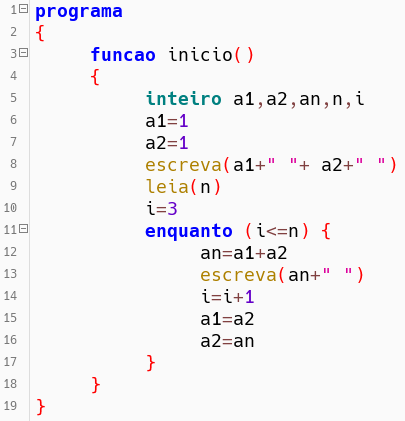
\includegraphics[width=.5\linewidth]{algoritmos10}
\end{figure}

\begin{reflection}
Você conhece essa sequência numérica?
\end{reflection}

O aspecto que é importante compreender neste algoritmo é o uso das variáveis \verb|i| e \verb|an|.

Note que a variável \verb|i| começa com o valor \verb|3| e ela aparece na condição que determina quantas vezes o comando enquanto vai ser repetido. Ao final dos comandos que são executados dentro do enquanto, o valor de \verb|i| é incrementado em \verb|1| unidade, até que ela fica maior do que n e o enquanto para de ser repetido. O papel dessa variável é servir como um contador para o enquanto.

Já a variável an tem uma função diferente. Para entendê-la, é necessário olhar para os comandos das linhas \verb|12|, \verb|15| e \verb|16| em conjunto. Na linha \verb|12|, a variável an recebe o valor de a1+a2 e depois o seu conteúdo é escrito, ou seja, \verb|an| é o próximo termo da sequência. Porém, o que ocorre nas linhas \verb|15| e \verb|16|?

\clearmargin
\begin{texto}
{\def\currentcolor{session2}
	Esta seção encerra a primeira parte do módulo sobre pensamento computacional. Como dito anteriormente, o objetivo desta parte era introduzir estratégias de pensamento computacional aos estudantes através de problemas matemáticos. Para tanto, propomos que estes problemas não sejam resolvidos como normalmente seriam abordados em aula, mas sob o ponto de vista computacional, com foco no processo de obtenção de suas soluções. Vimos nas seções anteriores como usar descrições verbais, fluxogramas e a linguagem de programação Portugol para criar algoritmos que resolvam problemas matemáticos e, para isso, estudamos usos comuns de variável, condicional e repetição.

	Nesta seção, são propostas quatro atividades cujas resoluções passam por tudo que foi estudado ao longo das seções anteriores, de modo que não é estritamente necessário resolver todas elas para completar os objetivos específicos desta parte. Elas podem ser discutidas em sala de aula, sem uso de dispositivo eletrônico que permita a execução dos algoritmos pedidos, uma vez que os problemas são matematicamente interessantes. Porém, o uso do laboratório poderá enriquecer o engajamento e potencializar o desenvolvimento do pensamento computacional dos seus estudantes, já que o uso do computador favorece o exercício de algumas habilidades ligadas a esse tipo de pensamento.

	As atividades são colocadas de maneira mais direta, deixando espaço para que o professor as desdobre no formato que achar mais adequado, dando mais ou menos ênfase para o lado computacional ou matemático. Por conta disso, não indicamos a duração de cada atividade nem a organização da turma, mas salientamos alguns aspectos que podem ser relevantes para o caso de uso em laboratório.

	Além disso, essas atividades também podem ser usadas para avaliação. Duas possibilidades para tal uso são:

	\begin{itemize}[topsep=0pt]
	\item Atividades em dupla ou em pequenos grupos de modo que as duplas devem escolher uma das quatro atividades e resolvê-la em um período de uma aula dupla;

	\item Dividir a turma em 8 grupos, de modo que cada atividade seja resolvida por 2 grupos diferentes. Os grupos deverão preparar uma apresentação curta e, a cada aula, os dois grupos que resolveram as mesmas atividades apresentarão suas resoluções.
	\end{itemize}

	Por fim, no \hyperref[comp-know1]{Para Saber Mais} é proposta uma atividade mais aberta que pode ser desdobrada em um projeto que ocuparia um número maior de aulas.
}
\end{texto}


O que está sendo feito ali é "avançando na sequência". Nesse ponto, as variáveis \verb|a1| e \verb|a2| deixam de ser o primeiro e segundo termos e passam a ser os próximos: \verb|a1| recebe o valor do \verb|a2| e \verb|a2| recebe o valor de \verb|an|, como se estivéssemos "andando"{} na sequência. Dessa forma, na próxima repetição, \verb|a1| e \verb|a2| serão os dois últimos valores calculados e an será a soma deles, ou seja, o próximo termo.

Você pode adaptar esse algoritmo, e o que aprendeu com as atividades anteriores, para obter outras sequências numéricas, como progressões aritméticas, progressões geométricas e os números triangulares. Pesquise na internet sobre essas sequências e tente construir algoritmos em Portugol para cada uma delas.

\practice{}
\label{comp-prac1}

Nesta seção, vamos praticar o que foi estudado até este momento. Todas as atividades propostas envolvem dois aspectos, o matemático e o computacional. Isso significa que conhecimentos matemáticos serão necessários para compreender e resolver os problemas e você também terá que pensar computacionalmente sobre o processo de resolução, ou seja, pensar sobre como transformar a resolução em um algoritmo.

\marginpar{\vspace{-1em}}
\begin{objectives}{Imposto de renda retido na fonte}
{
Compreender os conceitos básicos de uma linguagem de programação, como repetição, condicional e variáveis.
}{1}{1}
\end{objectives}

\marginpar{\vspace{-1em}}
\begin{sugestions}{Imposto de renda retido na fonte}
{
\textbf{Conexões}: a atividade tem conexões com funções definidas por partes e continuidade de funções, além de estar relacionada com tópicos abordados no módulo de Educação Financeira.

\textbf{Sugestão geral}: Você pode transformar essa atividade em uma proposta mais ampla, solicitando aos estudantes que pesquisem como o cálculo do imposto retido na fonte é feito e quais são as alíquotas e valores a deduzir para cada intervalo de salário bruto. Há muitas referências na internet que podem ser consultadas.

\textbf{Para o laboratório}: Como as variáveis usadas neste código são do tipo real, recomenda-se que ao atribuir um valor a elas, seja indicada ao menos uma casa decimal, mesmo que seja igual a 0, como na linha ir=0.0 na solução abaixo. Além disso, o Portugol pode considerar como erro as situações em que uma variável só recebe um valor dentro de comandos condicionais, pois caso a condição não seja satisfeita, o algoritmo poderia terminar sem que a variável receba um valor.

\textbf{Variações}: Você pode pedir que o algoritmo calcule o valor do salário após o desconto ou a alíquota efetivamente cobrada.
}{0}{9}
\end{sugestions}
\begin{answer}{Imposto de renda retido na fonte}
{
\begin{enumerate}
\item R\$ $0{,}00$, R\$ $95{,}20$ e R\$ $780{,}64$
\item \adjustbox{valign=t}
{
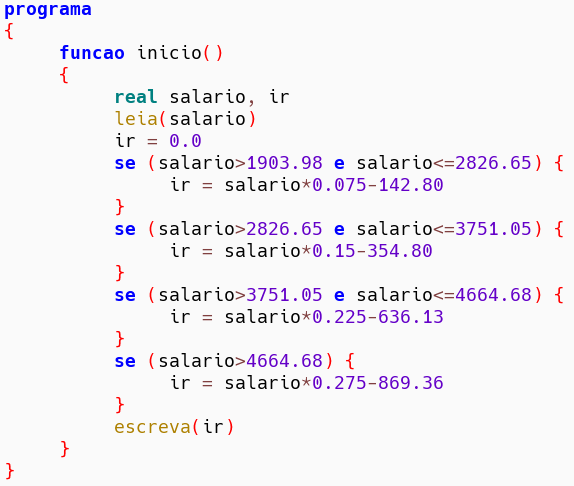
\includegraphics[width=.7\linewidth]{algoritmos6}
}
\end{enumerate}
}{1}
\end{answer}
\begin{objectives}{Xadrez}
{
Compreender os conceitos básicos de uma linguagem de programação, como repetição, condicional e variáveis.


}{1}{2}
\end{objectives}
\begin{sugestions}{Xadrez}
{
\textbf{Para o laboratório}: Este problema pode ser resolvido aritmeticamente com o auxílio do conceito de paridade (aplicada tanto às coordenadas de um dado quadradinho quanto à soma das coordenadas), mas admite soluções com repetições (em que o código alterna entre as duas soluções à medida que "percorre"{} um caminho até o quadradinho de destino). Incentive a discussão dessas duas soluções em termos de simplicidade, clareza e eficiência (qual delas obtém a solução realizando o menor número de operações?).

\textbf{Variação}: Você pode propor um tabuleiro diferente, em que as casas possuem três cores: branco, cinza e preto. Esse padrão se repete (nessa ordem) nas linhas e nas colunas (logo, a segunda linha começa em cinza e a terceira em preto). Nesse caso, a solução depende do uso do resto deixado na divisão por 3 e não de paridade.
}{1}{2}
\end{sugestions}
\begin{answer}{Xadrez}
{
\begin{enumerate}
\item Preto, branco, preto.
\item É possível resolver esta questão pensando na paridade da soma das dimensões (mostrado abaixo) ou na paridade das coordenadas isoladamente.

\item Várias soluções são possíveis, sendo essa uma delas:

\begin{figure}[H]
\centering

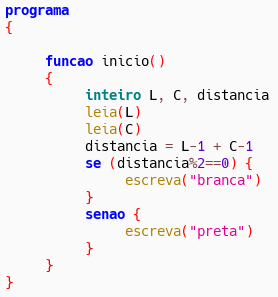
\includegraphics[width=.5\linewidth]{algoritmos7}
\end{figure}
\end{enumerate}
}{0}
\end{answer}
\begin{objectives}{MMC}
{
Compreender os conceitos básicos de uma linguagem de programação, como repetição, condicional e variáveis.
}{1}{1}
\end{objectives}
\begin{sugestions}{MMC}
{
\textbf{Comentários gerais}: Esta atividade reforça o uso de estruturas de repeticão através de um procedimento matemático conhecido, o cálculo do Mínimo Múltiplo Comum entre dois números. O problema pode ser resolvido com um algoritmo bastante curto, o que ilustra bem o poder dessas estruturas.

\textbf{Para o laboratório}: Um conceito computacionalmente muito importante que pode ser introduzido aos estudantes com este problema é o de função. Este conceito permite ao programador compartimentalizar um bloco de código que será usado para diferentes fins (vide este vídeo para um tutorial sobre funções em Portugol). Isso pode ser feito graças à conexão com máximo divisor comum sugerida no "Para Refletir": o algoritmo para obter o mínimo múltiplo comum pode ser transformado em uma função que será usada pelo algoritmo que calcula o máximo divisor comum.

\textbf{Variação}: Você pode pedir aos estudantes que usem as ideias desta atividade para construir um algoritmo que determine se dois números dados são coprimos, ou seja, se o MDC entre eles é igual a 1.
}{1}{1}
\end{sugestions}
\begin{answer}{MMC}
{
\begin{enumerate}
\item Vários métodos são ensinados para esse procedimento, mas os dois que parecem mais comuns envolvendo a listagem de múltiplos ou a fatoração simultânea dos dois números. Este último é computacionalmente mais eficiente, mas depende de uma lista de números primos para sua implementação.

\item \adjustbox{valign=t}
{
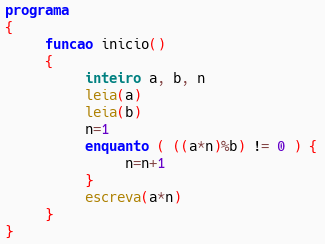
\includegraphics[width=.5\linewidth]{algoritmos8}
}

\item Basta acrescentar o cálculo sugerido pela propriedade ao final do algoritmo mostrado acima: "\texttt{mdc = (a*b)/(a*n)}".
\end{enumerate}
}{0}
\end{answer}
\begin{objectives}{Campeonato}
{
Compreender os conceitos básicos de uma linguagem de programação, como repetição, condicional e variáveis.
}{1}{1}
\end{objectives}
\begin{sugestions}{Campeonato}
{
\textbf{Comentários gerais}: Esta atividade propõe um problema matematicamente mais difícil do que todos os propostos até o momento. Além disso, ele pode ser resolvido algoritmicamente de diversas maneiras.

\textbf{Sugestões gerais}: A solução deste problema passa pela ideia de agrupamento dos números de 2 em 2 (se enfrentam na primeira fase), 4 em 4 (se enfrentam na segunda fase), 8 em 8 (se enfrentam na tercera fase) e assim por diante. Esse agrupamento pode ser detectado matematicamente verificando se a divisão das duas posições, menos 1, por 2, 4, 8 e 16 têm o mesmo resultado inteiro. Por exemplo, considere os times nas posições 3 e 8, como o quocitente de (3-1) e de (8-1) por 2 é diferente, eles não se enfrentam na fase 1, por 4 também, mas por 8 ambos têm quociente 0, logo, se enfrentam na fase 3.

\textbf{Para o laboratório}: É importante ter certeza de que os estudantes compreenderam a solução do ponto de vista matemático antes que tentem escrever a solução algorítmica. Outro aspecto importante se refere à forma como as posições são numeradas: se fossem de 0 a 15 e não de 1 a 16, a solução do problema seria mais direta.

\textbf{Variação}: Você pode aumentar o número de times participantes para 32, 64, etc. Isso pode levar à generalização do problema com  times participando.
}{1}{2}
\end{sugestions}
\begin{answer}{Campeonato}
{
A solução específica deste problema é mostrada abaixo. Curiosamente, ela é mais longa que a solução geral, porém, o significado das etapas do algoritmo são mais claras.

\centering
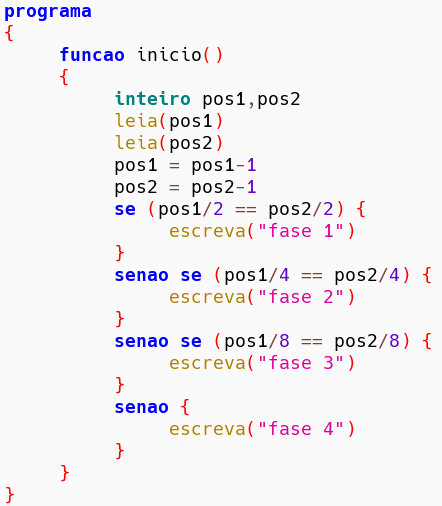
\includegraphics[width=.45\linewidth]{algoritmos11}
\justify

Uma solução geral, para  times participantes, é mostrada a seguir. A variável nfases permite que a solução seja ajustada para torneios com mais ou menos times participantes, desde que siga a mesma estrutura de chaves.

\centering
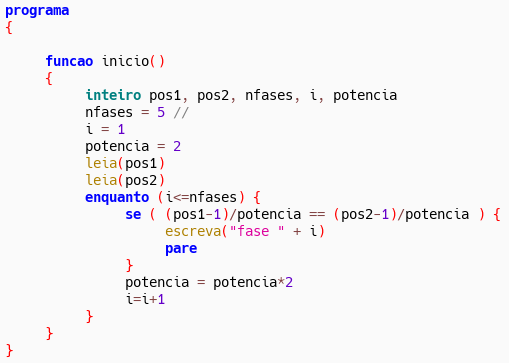
\includegraphics[width=.65\linewidth]{algoritmos9}
}{9}
\end{answer}

\begin{task}{Imposto de renda retido na fonte}

O imposto de renda é um dos principais impostos no Brasil. Uma das formas em que esse imposto é cobrado ocorre na folha de pagamento, ou seja, quando um funcionário com carteira de trabalho assinada recebe o seu salário. Essa forma de cobrança é chamada de imposto de renda retido na fonte. O cálculo do valor a ser descontado do salário (e imediatamente repassado ao governo federal) é feito de forma que ele seja percentualmente maior à medida que o salário aumenta. No Brasil, são adotados 5 intervalos de salário bruto (isto é, ainda sem o desconto do imposto) que seguem regras de cálculo diferentes. Para cada um desses intervalos, o cálculo é feito da seguinte maneira: calcula-se a porcentagem indicada em "alíquota"{} do salário bruto e, do resultado, subtrai-se a "parcela a deduzir". O resultado obtido é o valor que será descontado do salário no momento do pagamento.

\begin{table}[H]
\centering

\begin{tabular}{|l|c|r|}
\hline
\tcolor{Base de cálculo (R\$)} & \tcolor{Alíquota (\%)} & \tcolor{Parcela a deduzir do IR (R\$)} \\
\hline
Até $1.903{,}98$ & - & - \\
\hline
De $1.903{,}99$ até $2.826{,}65$ & 7,5 & $142{,}80$ \\
\hline
De 2$.825{,}55$ até $3.751{,}05$ & 15 & $354{,}80$ \\
\hline
$3.751{,}06$ até $4.664{,}68$ & 22,5 & $636{,}13$ \\
\hline
Acima de $4.664{,}68$ & 27,5 & $869{,}36$ \\
\hline
\end{tabular}
\caption{Fonte: \href{https://www.gov.br/receitafederal/pt-br/assuntos/orientacao-tributaria/tributos/irpf-imposto-de-renda-pessoa-fisica}{Receita Federal}}
\end{table}

Por exemplo, para um salário de R\$ $2.000{,}00$, começamos identificando que ele se encontra na segunda faixa. Logo, devemos calcular $7{,}5$\% de $2000$ e depois subtrair $142{,}80$ do resultado. Portanto, $0{,}075\times2000-142{,}80=7{,}20$ é o valor que será descontado do salário para pagar o imposto de renda desse trabalhador.

\begin{enumerate}
\item Quanto será descontado de uma pessoa que tenha salário bruto igual a R\$ $1.500{,}00$? E igual a R\$ $3.000{,}00$? E igual a R\$ $6.000{,}00$?

\item Crie um algoritmo que calcula o valor do imposto de renda a ser retido na fonte para um dado salário bruto.
\end{enumerate}

\end{task}

\begin{task}{Xadrez}
\textit{Fonte: Olimpíada Brasileira de Informática}
No tabuleiro de xadrez, a casa na linha 1, coluna 1 (canto superior esquerdo) é sempre branca e as cores das casas se alternam entre branca e preta. Dessa forma, como o tabuleiro tradicional tem oito linhas e oito colunas, a casa na linha 8, coluna 8 (canto inferior direito) será também branca. Neste problema, entretanto, queremos saber a cor da casa no canto inferior direito de um tabuleiro com dimensões quaisquer: L linhas e C colunas. No exemplo da figura, para L=6 e C=9, a casa no canto inferior direito será preta.

\begin{figure}[H]
\centering

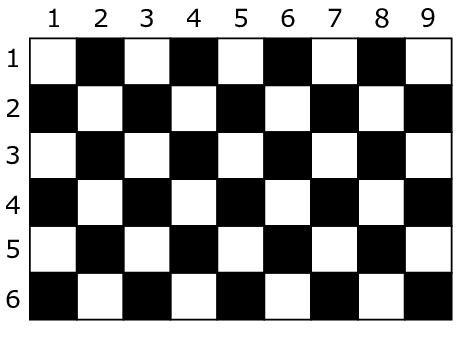
\includegraphics[width=.8\linewidth]{xadrez}
\end{figure}

\begin{enumerate}
\item Qual seria a cor da casa no canto inferior direito se o tabuleiro tiver 7 colunas e 4 linhas? E se tiver 10 colunas e 8 linhas? E se tiver 23 colunas e 40 linhas?

\item Descreva como descobrir a cor da casa no canto inferior direito de um tabuleiro como esse, sabendo a quantidade de linhas e colunas que o compõe.

\item Escreva um algoritmo que implemente o processo que você descreveu na questão anterior.
\end{enumerate}
\end{task}

\begin{task}{MMC}
Existem vários métodos para o cálculo do mínimo múltiplo comum (mmc) entre dois números inteiros. Você deve ter aprendido como fazer isso ainda no Ensino Fundamental e, de vez em quando, ainda deve utilizar esse procedimento para resolver algumas questões de matemática.

\begin{enumerate}
\item Descreva como você procede para obter o mínimo múltiplo comum entre dois números dados. Se quiser, comece obtendo o mínimo múltiplo comum para os números $12$ e $18$ e depois tente descrever o método que você utilizou de forma genérica, isto é, para dois números quaisquer $a$ e $b$.

Embora não seja o método mais eficiente, vamos implementar o método da lista. Ele consiste em listar os múltiplos do primeiro número (começando por ele mesmo) até encontrar um múltiplo que seja divisível pelo segundo número.

Exemplo: para o caso $12$ e $18$, vamos listar os múltiplos de $12$. Primeiro, o próprio $12$, que não é divisível por $18$. Depois $24$ $(12*2)$, que não é divisível por 18. Depois $36$ \verb|(12*3)|, que é divisível por 18 e, portanto, é o mínimo múltiplo comum entre esse $12$ e $18$.

\item Escreva um algoritmo que obtenha o mínimo múltiplo comum entre dois números naturais dados, usando o método da lista.
\end{enumerate}
\end{task}

\begin{reflection}
Sabendo como calcular o mínimo múltiplo comum entre dois números dados, $a$ e $b$, você pode utilizar uma propriedade simples para calcular o máximo divisor comum entre esses números. A propriedade diz que o máximo divisor comum entre $a$ e $b$ é igual ao produto dos dois números dividido pelo mínimo múltiplo comum entre eles:
 \begin{equation*}
\mdc(a,b)=\frac{a\cdot b}{\mmc(a,b)}
\end{equation*}
Como você poderia usar essa propriedade para escrever um algoritmo que obtenha o máximo divisor comum entre dois números naturais dados.
\end{reflection}

\begin{task}{Campeonato}
Um torneio esportivo mundial é organizado no tradicional formato de chaves: dois competidores se enfrentam e quem vence passa para a próxima etapa, até que os dois que venceram todas as partidas se enfrentem na final. Nesta edição, o torneio vai contar com 16 competidores e os confrontos ocorrerão como mostrado abaixo.

\begin{figure}[H]
\centering

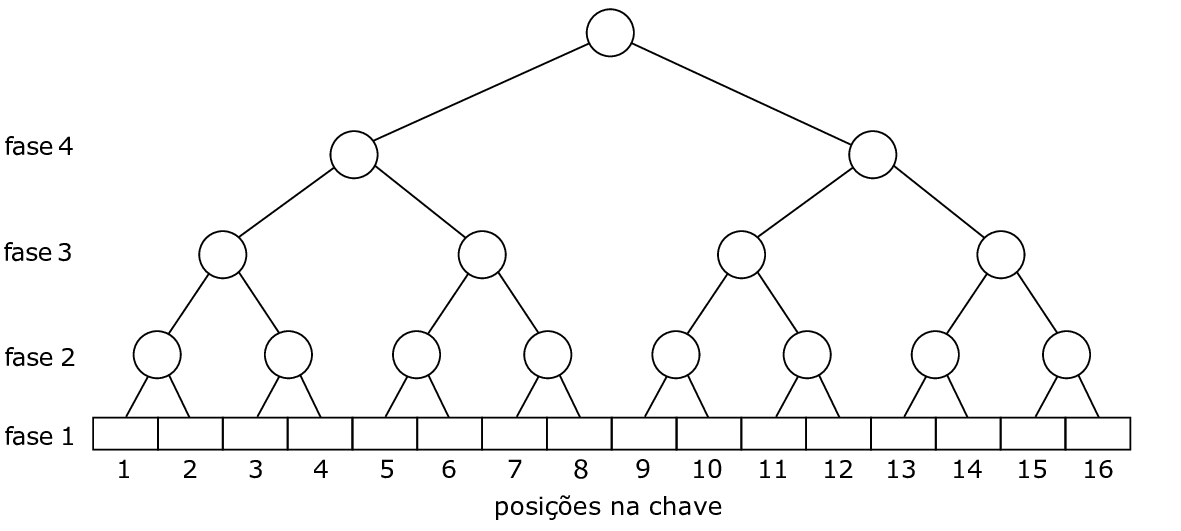
\includegraphics[width=\linewidth]{campeonato}
\end{figure}

O grande adversário do Brasil neste torneio é os Estados Unidos e, por isso, todos querem saber quando os competidores desses dois países poderão vir a se enfrentar. Isso será determinado um dia antes do início do torneio, quando será sorteada uma bolinha com um número de 1 a 16 para cada país, indicado a posição em que eles serão alocados nas chaves.

Escreva um algoritmo que, dadas as duas posições do Brasil e Estados Unidos nas chaves, determina em qual fase do torneio os países poderão se enfrentar.
\end{task}

\begin{reflection}
Você conseguiria modificar o seu algoritmo de modo que ele possa ser usado para outras quantidades de competidores?

Você pode assumir que essas quantidades sempre serão uma potência de $2$ ($2, 4, 8, 16, 32, 64$, etc).
\end{reflection}

\know{Um projeto com bolinhas e vetores}
\label{comp-know3}

\clearmargin
\begin{texto}
{
Professor, esta atividade foi proposta com o objetivo de oferecer um problema desafiador e interessante, mas ainda acessivel para os estudantes que tenham sido bem sucedidos nas atividades propostas na seção Praticando. A atividade deve ser encarada como um projeto, que exigirá uma maior dedicação de tempo dos estudantes.

Do ponto de vista computacional, o problema oferece uma oportunidade interessante para que os estudantes aprendam a utilizar vetores. Do ponto de vista matemático, o problema pode ser relacionado com álgebra booleana (ao pensarmos nas cores como os valores 0 e 1) e, surpreendemente, com o Triângulo de Pascal.

Uma referência sobre este problema, discutindo a sua solução matemática e computacional, pode ser encontrada em \url{doi.org/10.1080/0020739X.2015.1109147} (em inglês).
}
\end{texto}

Para o encerramento desta parte, escolhemos um problema que foi sugerido na Olimpíada Brasileira de Informática. Este problema, além do desafio matemático envolvido na sua resolução, vai exigir que você aprenda um novo conceito muito importante em todas as linguagens de programação. Mas vamos começar com o problema.

\textbf{Triângulo de bolinhas}: Dois amigos inventaram um passatempo com bolas pretas e brancas. Elas são colocadas uma por vez na mesa, de acordo com uma regra fixa: no início, são colocadas N bolas formando a primeira fileira; em seguida, um triângulo é formado, fileira a fileira, de modo que ao se colocar uma bola na nova fileira, ela ficará encostada em duas bolas da fileira anterior e sua cor será:

\begin{itemize}
\item Preta, se estiver encostada em duas bolas de mesma cor;
Branca, se estiver encostada em duas bolas de cores diferentes.

\item O passatempo acaba quando a bolinha do topo é colocada. A figura abaixo ilustra a formação de um triângulo para N=5.
\end{itemize}

\begin{figure}[H]
\centering

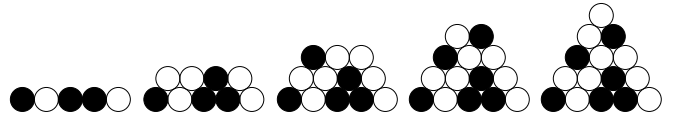
\includegraphics[width=\linewidth]{sinuca}
\end{figure}

A partir deste contexto, é possível colocar várias perguntas que podem ser respondidas com auxílio da matemática e da computação. Por exemplo:

\begin{itemize}
\item Dadas as cores das bolinhas da primeira linha, qual será a cor da bolinha do topo?
\item É possível prever a cor da última bolinha sem precisar construir todas as linhas?
\end{itemize}
A criação de algoritmos que permitam a investigação dessas perguntas depende do uso de um recurso existente em todas as linguagens de programação, mas que não discutiremos neste livro. Este recurso é chamado vetor em português, ou array em inglês. Ele tem algumas semelhanças com o conceito de vetor que são estudadas nas aulas de matemática e física, mas seu uso em computação tem algumas peculiaridades que precisam ser compreendidas para seu uso efetivo. De maneira simplificada, um vetor é uma variável que contém várias variáveis de um mesmo tipo dentro e essas variáveis podem ser acessadas de acordo com a sua posição no vetor. Você pode aprender mais sobre vetores em Portugol com o vídeo \url{youtu.be/5oQrDq8qqfg}.

Nossa sugestão é que este problema seja encarado como um projeto, ou seja, que não será resolvido em uma ou duas aulas, mas exigirá de você (e de seus colegas) muito estudo, análises e discussões. Bom trabalho!

\begin{paginatexto}{Parte II}

\subsection{Apresentação}
As atividades desta seção foram escolhidas para que os estudantes tenham experiência em usar uma linguagem de programação para explorar problemas matemáticos, ou seja, como uma ferramenta que permite simular, testar casos, realizar cálculos de maneira rápida e precisa, gerar dados, etc.

Em linhas gerais, as atividades desta parte promovem a habilidade \textbf{EM13MAT405} (Utilizar conceitos iniciais de uma linguagem de programação na implementação de algoritmos escritos em linguagem corrente e/ou matemática) e reforçam a habilidade \textbf{EM13MAT315} (Investigar e registrar, por meio de um fluxograma, quando possível, um algoritmo que resolve um problema), que foi desenvolvida na parte anterior. Além disso, as atividades promovem a integração do pensamento computacional e da programação ao currículo regular de matemática, atendendo ao \textbf{Objetivo Específico 4} (Aplicar o pensamento computacional e formas sistemáticas de representação de um algoritmo para criar soluções para problemas relacionados a conteúdos matemáticos) e reforçando o \textbf{Objetivo Específico 3} (Compreender os conceitos básicos de uma linguagem deprogramação, como repetição, condicional e variável).

Também é importante salientar que as atividades propostas nesta seção partem do pressuposto de que exista um laboratório de informática disponível para uso por, pelo menos, uma aula por atividade. O uso de computadores é recomendável nesta parte, já que o foco é usá-los como ferramenta para resolver problemas matemáticos. Entretanto, pode ser possível organizar a turma de modo que as atividades sejam realizadas em celulares ou com um número reduzido de computadores.

\subsection{Dois usos diferentes}

Diferentemente da parte anterior, que deve ser vista como um capítulo a ser estudado do início ao fim, esta parte pode ser usada de duas formas diferentes.

A primeira delas é como um capítulo convencional a ser estudado após a primeira parte deste módulo. Nesse caso, as atividades propostas servem como aplicação do que foi aprendido anteriormente, mas dependem de um conhecimento mais aprofundado dos tópicos matemáticos envolvidos.

A segunda possibilidade de utilização que vislumbramos é de forma integrada aos demais módulos. Nesse cenário, sugerimos que a primeira parte seja estudada no início no primeiro ano letivo do Ensino Médio, para que os estudantes desenvolvam o pensamento computacional e dominem alguns conceitos de linguagem de programação. Depois, ao invés de resolver as atividades desta parte sequencialmente, sugerimos que o professor espere a discussão dos tópicos matemáticos relacionados e, então, traga estas atividades para a sala de aula.

Essa segunda abordagem nos parece mais promissora no sentido de integrar o pensamento computacional de maneira mais orgânica na disciplina de Matemática, como recomendado por \citet{disessa2018} e \citet{li2020}. Entretanto, ela demanda uma certa flexibilidade curricular para encaixar a primeira parte do módulo no início do Ensino Médio e incluir as ativdades desta parte ao longo dos demais módulos.

\subsection{As atividades}
Abaixo, apresentamos o resumo de cada uma das atividades, dando especial atenção à relação da mesma com os demais módulos do Livro Aberto. A ordem em que elas são apresentadas foi definida pela dificuldade computacional, mas não precisa ser seguida.

Números binários: nesta atividade discutimos a representação de números na base 2, ou seja, usando apenas 0s e 1s, como ocorre internamente em computadores. Do ponto de vista matemático, o conteúdo se relaciona com sistemas de numeração, especificamente com o sistema de numeração binário, potências de 2 e com contagem. Mais espeficamente, a atividade dialoga com a questão sobre o sistema de escrita Braile proposta no módulo sobre Contagem. Do ponto de vista computacional, a atividade explora repetições, condicionais e cálculos com variáveis. As habilidades desenvolvidas são: \textbf{EM13MAT405} e \textbf{EM13MAT310}.

Quantas caras: nesta atividade propomos um jogo com moedas e discutimos como construir um simulador em Portugol para o jogo. Com esse simulador, não apenas os estudantes poderão simular muitas jogadas e analisar os resultados obtidos, mas também explorar pequenas variações do jogo de forma empírica. A proposta dialoga com o Para Saber Mais proposto no final do módulo de Probabilidade, onde os autores sugerem a simulação do lançamento de uma moeda com o auxílio de planilhas eletrônicas. Do ponto de vista computacional, a atividade explora basicamente repetições e condicionais simples. As habilidades desenvolvidas são: \textbf{EM13MAT405} e \textbf{EM13MAT511}.

Método da bissecção: no Para Saber Mais entitulado "Sem ferramentas de Cálculo", do módulo sobre logaritmos, foi introduzido o método da bissecção para determinar o valor aproximado de . Nesta atividade, vamos mostrar como implementar esse método em Portugol e, por se tratar de um método polivalente, ele poderá ser utilizado para encontrar aproximações para outros números irracionais. A habilidade desenvolvida é: \textbf{EM13MAT405}.

Tem sinal?: nesta atividade, propomos uma questão de interesse atual: dada uma posição e um conjunto de torres que transmitem algum tipo de sinal, há sinal disponível nessa posição? O problema é tratado no plano e envolve conceitos geométricos como distância entre pontos e definição de circunferência, assim como trabalha a ideia de inequação. Do ponto de vista de programação, o problema não é complexo e exige apenas alguns cálculos juntamente com condicionais e repetições simples. A habilidade desenvolvida é: \textbf{EM13MAT405}.

\subsection{Avaliação}

Todas as seções trazem, nas notas para o professor, sugestões de variações das atividades propostas que podem ser usadas para fins de avaliação.
\end{paginatexto}

\def\currentcolor{session1}
\begin{texto}
{
Nesta seção propomos uma investigação sobre a representação binária de números a partir da discussão que foi feita na atividade sobre o alfabeto Braile, no módulo sobre Contagem. A discussão aqui enfatizará o aspecto numérico do conteúdo, e não aspectos de análise combinatória, mas acreditamos que o aprofundamento dessa discussão pode contribuir com um entendimento mais profundo do contexto como um todo. O objetivo final da seção é construir um algoritmo que converta um número dado na base decimal para a base binária.

Como um todo, esta seção leva 2 aulas para ser realizada, sem considerar as sugestões deixadas no \hyperref[comp-know1]{Para Saber Mais}.

Sugerimos, na introdução, o vídeo Hit dos Bits, da coleção \href{https://m3.ime.unicamp.br/}{Matemática Multimídia}. O vídeo faz uma apresentação geral do sistema de númeração binário, mas caso a sua utilização não seja viável, o professor pode fazer a introdução expositivamente a partir das questões propostas.

Do ponto de vista matemático, os conteúdos utilizados aqui são simples: potências de 2, somas e subtrações. Do ponto de vista computacional, utilizaremos repetições e condicionais para atingir o objetivo final.

Esta seção tem um relevância maior para o contexto computacional por conta do uso da base binária na representação de informações por computadores.

\textbf{Habilidades}: \textbf{EM13MAT405} (Utilizar conceitos iniciais de uma linguagem de programação na implementação de algoritmos escritos em linguagem corrente e/ou matemática) e \textbf{EM13MAT310} (Resolver e elaborar problemas de contagem envolvendo agrupamentos ordenáveis ou não de elementos, por meio dos princípios multiplicativo e aditivo, recorrendo a estratégias diversas, como o diagrama de árvore).

}
\end{texto}
\clearmargin
\begin{objectives}{Dois estados}
{
\begin{itemize}
\item O objetivo principal desta atividade é familiarizar os estudantes com a base binária e com o método de conversão de um número dado na base decimal para a base binária que será usado para criar o algoritmo final.

\item Aplicar o pensamento computacional e formas sistemáticas de representação de um algoritmo para criar ~soluções para problemas relacionados a conteúdos matemáticos
\end{itemize}
}{1}{2}
\end{objectives}
\begin{sugestions}{Dois estados}
{
\textbf{Duração}: 1 aula, incluindo a discussão do explorando logo em seguida.

\textbf{Organização da turma}: sugerimos a divisão da turma em duplas.
}{1}{2}
\end{sugestions}
\begin{answer}{Dois estados}
{
\begin{enumerate}[left=1.5em]
\item $5, 16$ e $3$.

\item $1010, 11001 \text{ e } 110010$.

\item[\titem{c)} e \titem{d)}] Nesta questão, não esperamos que os estudantes obtenham um algoritmo bem estruturado e claro para o processo. Isso é apresentado logo depois da atividade. A dinâmica sugerida na questão 3 deve ser suficiente para mostrar a eles pontos que podem ser melhorados nas suas respostas
\end{enumerate}
}{1}
\end{answer}
\clearmargin
\clearmargin
\begin{objectives}{0s e 1s}
{
Aplicar o pensamento computacional e formas sistemáticas de representação de um algoritmo para criar soluções para problemas relacionados a conteúdos matemáticos.
}{1}{2}
\end{objectives}
\begin{sugestions}{0s e 1s}
{
\textbf{Duração}: 1 aula no laboratório de informática.

\textbf{Enriquecimento da discussão}: uma vez obtido o algoritmo, você pode propor perguntas adicionais para os estudantes de modo a investigar algumas propriedades dos números escritos na base $2$. Alguns exemplos são: como podemos identificar números pares e ímpares na base $2$? O que acontece com a representação binária de um número quando dobramos o seu valor? Você observa algum padrão nos algarismos da representação binária dos números de $0$ a $31$?
}{1}{2}
\end{sugestions}
\begin{answer}{0s e 1s}
{
\begin{enumerate}
\item 10010001
\item \adjustbox{valign=t}
{
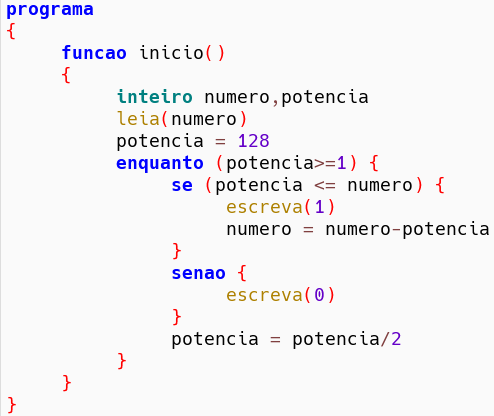
\includegraphics[width=.7\linewidth]{p2_binarios_2}
}
\end{enumerate}
}{1}
\end{answer}
\explore{Números binários}
\label{comp-exp6}
\subsection{Dois estados}

Na atividade sobre alfabeto Braile no módulo sobre Contagem, você conheceu um pouco sobre esta forma de escrita desenvolvida para cegos. Basicamente, você viu que as letras em Braile são representadas por um conjunto de 6 pontos dispostos em 2 colunas e 3 linhas, de modo que o estado de cada ponto pode ser marcado (pontos maiores na figura abaixo, em relevo quando impressos) ou não marcado (pontos menores na imagem abaixo, sem relevo quando impressos).

\begin{figure}[H]
\centering

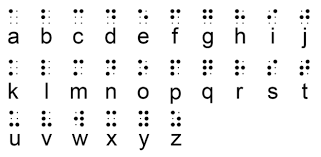
\includegraphics[width=.5\linewidth]{p2_binarios_1}
\end{figure}

A questão resolvida no módulo sobre Contagem foi: quantos caracteres diferentes podemos montar com a estrutura do alfabeto Braile?

Para resolver a esta questão, usamos basicamente a ideia de que cada pontinho é independente e pode assumir dois estados: com relevo ou sem relevo. Dessa forma, para cada um dos 6 pontinhos temos duas possibilidades, o que leva a: $2\cdot2\cdot2\cdot2\cdot2\cdot2=2^6=64$ caracteres ($63$ se excluírmos o caso em que nenhum pontinho foi marcado).

O que vamos explorar nesta seção é uma relação do alfabeto Braile com a maneira como computadores guardam informação.

A relação vem de outra característica: assim como o alfabeto Braile, computadores utilizam apenas dois estados para armazenar informações, os famosos 0 e 1 (ligado e desligado, carregado e descarregado, verdadeiro e falso, etc).

O vídeo \href{https://m3.ime.unicamp.br/recursos/1116}{Hit dos Bits}, da coleção Matemática Multimídia explica como o sistema de representação binário é usado por computadores.

Nesta seção, vamos analisar o sistema de representação binária com o objetivo de escrever um algoritmo que converta um número dado na base decimal para a base binária. Mas para isso, é importante compreendermos bem como essa conversão funciona.

\clearpage
\begin{task}{Dois estados}
No sistema de numeração decimal, ou de base $10$, cada algarismo de um número, como o $308$, representa um múltiplo de uma potência de $10$:

\begin{align*}
308&=300+0+8\\
308&=3\cdot100+0\cdot10+8\cdot1\\
308&=3\cdot10^2+-\cdot10^1+8\cdot10^0
\end{align*}
 
No sistema de numeração binário, ou de base $2$, temos apenas dois algarismos disponíveis, o $0$ e o $1$, e a posição de cada algarismo determina qual potência de $2$ ele está multiplicando. Por exemplo, o número $1101$, na representação binária, pode ser convertido para a base decimal da seguinte forma:

 
\begin{enumerate}
\item Usando essas ideias, obtenha a representação decimal dos seguintes números dados em representação binária: $101$, $10000$ e $11$.

O processo descrito acima é relativamente simples, pois ao escrevermos as potências de $2$ já estamos trabalhando na representação decimal, na qual sabemos fazer somas e multiplicações sem dificuldades. Já o processo inverso, de transformar um número dado na representação decimal para a representação binária, é um pouco mais difícil, pois precisamos encontrar quais potências de $2$ compõem o número em questão.

Por exemplo, o $20$ pode ser escrito com $16+4$. Note que $16$ e $4$ são ambos potências de $2$, $16=2^4$ e $4=2^2$. Logo:
 
\begin{align*}
20&=16+4\\
20&=2^4+2^2\\
20&1\cdot2^4+1\cdot2^2\\
20&1\cdot2^4+1\cdot2^2\\
20&1\cdot2^4+0\cdot2^3+1\cdot2^2+0\cdot2^1+0\cdot2^0
\end{align*}

Assim, o número $20$ é representado na base binária por $10100$.

\item Escreva os números $10$, $25$ e $50$ na base binária, como mostrado no exemplo anterior e seguindo a estrutura da tabela abaixo.

\begin{table}[H]
\centering

\begin{tabular}{|e{.175\linewidth}|e{.15\linewidth}|c|e{.175\linewidth}|}
\hline
\tcolor{Representação decimal} & \tcolor{Soma de potências de $2$} & \tcolor{Soma completa de potências de $2$} & \tcolor{Representação binária} \tabularnewline
\hline
$20$ & $16+4$ & $1\cdot2^4+0\cdot2^3+1\cdot2^2+0\cdot2^1+0\cdot2^0$ & $10100$ \tabularnewline
\hline
$10$ & & & \tabularnewline
\hline
$25$ & & & \tabularnewline
\hline
$50$ & & & \tabularnewline
\hline
\end{tabular}
\end{table}

Agora, vamos pensar sobre esse procedimento de forma a sistematizá-lo em um algoritmo.

\item Tente descrever textualmente, ou com auxílio de um fluxograma, como você pode proceder para converter um número natural dado na representação decimal para a representação binária. Faça essa descrição em uma folha de papel avulsa com a frente e o verso em branco.

\item Troque com um colega a sua descrição e avalie se você consegue seguir as instruções criadas por ele e se elas funcionam corretamente. Faça anotações para o seu colega, destroque e reescreva a sua descrição no verso da folha levando em conta as anotações feitas na sua descrição pelo seu colega.
\end{enumerate}
\end{task}

\subsection{0s e 1s}

Existe mais de uma maneira de converter um número inteiro da base decimal para a base binária e o método que vamos utilizar se baseia em encontrar quais potências de 2 são menores do que o número que se deseja representar.

Para entender essa abordagem, precisamos levar em conta uma propriedade das potências de 2. Essa propriedade diz que a soma das potências de $2$ até uma determinada potência  é menor do que a próxima potência de $2$. Isto é, $2^0+2^1+2^2+2^3+\dots+2^n<2^{n+1}$.

Não demonstraremos essa propriedade aqui, mas isso pode ser feito com auxílio de progressões geométricas.

O que essa propriedade nos permite concluir é que se uma potência de $2$ é menor do que um determinado número, ela necessariamente deve aparecer na representação binária desse número. Vejamos um exemplocom o número $46$.

Começamos listando as potências de $2$ até que elas sejam maiores do que $46$: $1$, $2$, $4$, $8$, $16$, $32$ e $64$. Como $64$ é maior do que $46$, ele não vai entrar na representação binária desse número. Mas como $32$ é menor, ele vai entrar. Podemos escrever o seguinte:

\begin{equation*}
46=32+14=2^5+14
\end{equation*}

Agora, temos que continuar o processo com a parte que ainda não é uma potência de $2$, ou seja, o $14$. Como a maior potência de $2$ menor do que $14$ é $8$, escrevemos o $14$ como uma soma de 8 mais a diferença, no caso, $6$:

\begin{align*}
46&=2^5+14 \\
46&=2^5+(8+6) \\
46&=2^5+2^3+6 \\
\end{align*}
 
O processo continua até termos apenas potências de $2$ na soma.

\begin{align*}
46&=2^5+14 \\
46&=2^5+(8+6) \\
46&=2^5+2^3+6 \\
46&=2^5+3^3+(4+2) \\
46&=2^5+2^3+2^2+2^1
\end{align*}
 
Finalmente, indicando o 1 como multiplicador de cada uma das potências acima e completamos com as potências de 2 que não apareceram multiplicando-as por 0 (para não alterar o valor da soma:

\begin{align*}
46&=2^5+2^3+2^2+2^1 \\
46&=1\cdot2^5+1\cdot2^3+1\cdot2^2+1\cdot2^1 \\
46&=1\cdot2^5+0\cdot2^4+1\cdot2^3+1\cdot2^2+1\cdot2^1+0\cdot2^0
\end{align*}
 
Portanto, a representação binária de $46$ é dada por $101110$.

\begin{task}{0s e 1s}
\begin{enumerate}
\item Use o procedimento descrito acima para obter a representação binária do número $145$.

\item Escreva em Portugol um algoritmo que converta um número inteiro, dado na base decimal, para a base binária. Vamos assumir, por enquanto, que o número dado é menor do que $256$, ou seja, você precisa considerar apena as potências de $2$ até $2^7$.

\item Use o algoritmo obtido na questão anterior para obter a representação decimal do número $200$.
\end{enumerate}
\end{task}

\arrange{0s e 1s}
\label{comp-arr6}

A base binária é importante não apenas pelo seu uso em computação, mas também pela sua simplicidade: o fato de usarmos apenas 2 símbolos (0s e 1s) para representar um número qualquer confere a ela algumas propriedades que podem ser usadas em diversos outros contextos.

Em contagem, é possível fazer analogias muito interessantes entre a base binária e o processo de escolher  elementos de um conjunto de  elementos disponíveis, pois podemos pensar que cada elemento admite dois estados: ser ou não ser escolhido.

Considere o seguinte cenário: queremos escolher 2 letras dentre as letras $A, B, C, D \text{ e } E$. Podemos traduzir as escolhas para o seguinte formato:

\begin{itemize}
\item Escolher $A$ e $B$ pode ser representado como $1,1,0,0,0$
\item Escolher $C$ e $E$ pode ser representado como $0,0,1,0,1$
\item Escolher $A$ e $D$ pode ser representado como $1,0,0,1,0$
\end{itemize}

Nessa representação, $1$ significa "escolhido"{} e "$0$"{} significa "não escolhido"{} e todos os elementos disponíveis devem ser marcados em um dos dois estados.

Note que agora cada escolha pode ser vista como um número de 5 algarismos na base binária. Portanto, para saber de quantas formas podemos fazer essa escolha, basta contar quantos números binários de $5$ algarismos são representados exatamente com dois algarismos $1$.

Esse é apenas um dos exemplos fora da computação e da escrita em Braile em que podemos aplicar a base binária.


\know{Outras bases}
\label{comp-know4}

Mas não só das bases decimal e binária vive o mundo atual!

Em contextos digitais, cores são comumente representadas na base 16 (hexadecimal). Nessa base, além dos algarismos $0, 1, 2, 3, 4, 5, 6, 7, 8$ e $9$, são usadas as letras $A, B, C, D, E$, e $F$, totalizando $16$ opções.

Por exemplo, a cor conhecida como "verde militar"{} é dada pela seguinte trinca de números em hexadecimal: $78 86 6b$. Essa trinca representa a quantidade de vermelho ($78$), verde ($86$) e azul ($6b$) que devem ser usadas para compor a cor desejada. Na verdade, o código que representa cores é usualmente apresentado com um "\#"{} na frente e sem nenhum espaço entre as três quantidades, ou seja, verde militar será dado por "$\#78866b$". \href{https://www.youtube.com/watch?v=uuUzkqSxCz4}{Neste vídeo}, você pode aprender um pouco mais sobre a base hexadecimal.

A base 3 é pouco utilizada em contexto digitais, mas aparece de forma natural em um problema concreto: como encontrar um saquinho mais leve em um conjunto de saquinhos que deveriam ter exatamente o mesmo peso com o auxílio de uma balança de braços? O problema, a resolução e a sua relação com a base 3 são apresentados no texto \href{http://rpm.org.br/cdrpm/79/4.html}{Balança e a base 3}.


\explore{O método da bissecção}
\label{comp-exp7}
\def\currentcolor{session1}
\begin{texto}
{
Nesta seção criamos e discutimos um algoritmo que implemente o método da bissecção apresentado no módulo sobre logaritmos do Livro Aberto de Matemática. A intenção é aproveitar o contexto criado nesse outro módulo para desenvolver alguns aspectos ligados a pensamento computacional e linguagens de programação e, também, discutir a questão do erro e aproximações. Nesse caso, sugerimos que a questão sobre $\log_25$ posta no final do \textbf{Para Saber Mais} seja reservada para ser resolvida ao longo desta seção.

Do ponto de vista matemático, o conteúdo necessário para a atividade que propomos é mais simples do que o conteúdo que foi utilizado na discussão sobre o método da bissecção proposta no módulo sobre logaritmos, pois os estudantes não precisarão fazer manualmente a comparação de potências com expoentes fracionários.

Além do algoritmo, no \textbf{Organizando} que encerra esta parte, trazemos uma discussão sobre erros e aproximações. Sugerimos que essa parte seja discutida em sala de aula, pois não há necessidade de os alunos usarem seus próprios algoritmos. Essa discussão não é realizada em outros módulos do Livro Aberto e pouco feita em nível de Ensino Médio, apesar de ser muito pertinente para a discussão dos números reais.

Do ponto de vista da computação, o algoritmo faz uso de cálculos e repetições relativamente simples. A novidade introduzida aqui é o uso de bibliotecas em Portugol, algo bastante útil e comum no universo de programação de computadores.

\textbf{Habilidades}: \textbf{EM13MAT405} (Utilizar conceitos iniciais de uma linguagem de programação na implementação de algoritmos escritos em linguagem corrente e/ou matemática).
}
\end{texto}
\clearmargin
\begin{objectives}{Implementando o método da bissecção}
{
Aplicar o pensamento computacional e formas sistemáticas de representação de um algoritmo para criar soluções para problemas relacionados a conteúdos matemáticos.
}{1}{2}
\end{objectives}
\begin{sugestions}{Implementando o método da bissecção}
{
\textbf{Duração}: 1 aula, sem considerar as discussões propostas no Organizando a seguir.

\textbf{Organização da turma}: sugerimos a divisão da turma em grupos pequenos ou em duplas, de acordo com a disponibilidade de computadores.
}{1}{2}
\end{sugestions}
\begin{answer}{Implementando o método da bissecção}
{
\begin{enumerate}
\item Pode haver alguma variação em como os estudantes contam a primeira repetição (começando em 0 ou 1), em como eles obtém o primeiro valor médio (antes da repetição ser iniciada ou dentro dela) e como lidam com a última repetição (calculando o último valor médio dentro ou depois da repetição).

\item \adjustbox{valign=t}
{
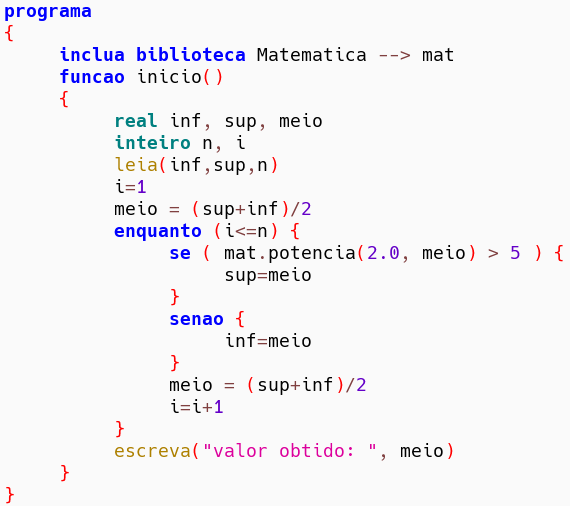
\includegraphics[width=.7\linewidth]{p2_bisseccao_3}
}

\item $2{,}265625$ e $2{,}32275390625$.

\item Basta alterar a condição do comando se para obter essas variações.
\end{enumerate}
}{1}
\end{answer}

\subsection{Usando o computador para calcular $\log_25$}

No módulo sobre Logaritmos, você viu o método da bissecção sendo aplicado para calcular uma aproximação para $\log_23$. O método foi descrito da seguinte maneira:

\begin{observationtitle}{Método da bissecção}
Para aplicarmos o método da bissecção, tomamos uma aproximação superior e outra inferior para o número buscado, encontrando assim um intervalo no qual temos certeza que a solução se encontra. Então tomamos o ponto médio desse intervalo como a próxima aproximação e buscamos decidir se ele é superior ou inferior ao número buscado, daí basta substituirmos o respectivo extremo do intervalo pelo ponto médio. Repetindo esse processo obtemos aproximações cada vez melhores.
\end{observationtitle}

Logo em seguida, uma aplicação do método no cálculo de uma proximação para $\log_23$ é apresentada em detalhes. O que faremos nesta seção é implementar um algoritmo que execute este método pensando, inicialmente, em $\log_25$.

Porém, para isso, você precisa aprender antes a usar uma nova funcionalidade do Portugol chamada \textbf{biblioteca}. Uma biblioteca é um conjunto de comandos que não estão disponíveis entre as funcionalidades básicas de uma linguagem de programação. Esse é o caso do comando que calcula o valor de um número real elevado a outro número real, ou seja, . Para realizar esse cálculo, precisamos de uma função que faz parte da biblioteca chamada Matematica no Portugol. Veja no código abaixo como essa biblioteca é carregada e usada.

\begin{figure}[H]
\centering

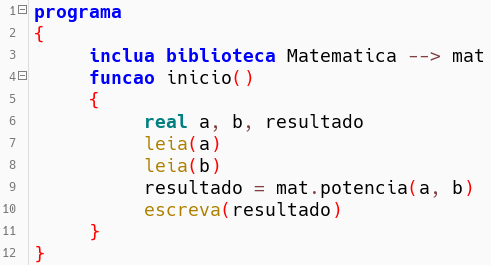
\includegraphics[width=.5\linewidth]{p2_bisseccao_1}
\end{figure}

O comando usado na linha 3 carrega os comandos que fazem parte dessa biblioteca na variável \verb|mat|. Na linha 9, o comando \verb|potencia| é usado, mas como ela faz parte da biblioteca, ele precisa ser acionado não apenas pelo seu nome, mas acrescentando \verb|mat|. logo antes. Isso diz ao computador para usar o comando potencia que está carregado na variável \verb|mat|.

\begin{reflection}
A possibilidade de usarmos esse comando poupa as várias comparações feitas no módulo sobre logaritmos com as potências de expoente fracionário. Isso é conveniente no sentido de economizar cálculos, mas é importante estarmos atentos quanto às saídas apresentadas, a fim de verificarmos que elas correspondem à programação prentendida.
\end{reflection}


\begin{task}{Implementando o método da bissecção}
\begin{enumerate}
\item Leia a descrição do método da bissecção dada acima e, se necessário, o exemplo dado no módulo sobre logaritmos e descreva textualmente, por meio de um fluxograma, o método da bissecção para obter uma aproximação para o valor de $\log_25$.

\item Escreva um algoritmo em Portugol implementando a resposta da questão anterior. Seu algoritmo deve pedir ao usuário quantas repetições ele deseja fazer e quais são os valores inferior e superior iniciais. Ao final, seu algoritmo deve mostrar o último valor médio calculado.

\item Se usarmos $5$ repetições e $1$ e $10$ como valores inferior e superior iniciais, qual é o valor que o seu algoritmo obtem para $\log_25$? E se usarmos 10 repetições?

\item Use o seu algoritmo para gerar aproximações para $\log_27$ e $\log_{10}2$. Qual valor você obteve?
\end{enumerate}
\end{task}

\begin{reflection}
Quais alterações devem ser feitas no seu algoritmo para que ele obtenha aproximações para $\sqrt{2}$?
\end{reflection}

\arrange{Aproximação, erro e estimativa do erro}
\label{comp-arr7}

O uso que fizemos do método da bissecção permite-nos encontrar a representação decimal de $\log_25$, com o número de casas de precisão que se desejar, supondo que sabemos como calcular potências de 2. O Portugol também apresenta na biblioteca matematica a função logaritmo, que calcula o valor de $\log_25$ diretamente, mas o nosso objetivo ao apresentar o método da bissecção é obter a representação decimal de um número com a precisão que se quiser.

É importante estarmos cientes de que métodos como os da bissecção obtêm aproximações para os valores buscados. Essas aproximações tornam-se cada vez mais precisas à medida que aumentamos o número de repetições. Para ilustrar esse fenômeno, vamos usar o algoritmo abaixo. Leia-o com atenção antes de utilizá-lo para ter certeza de que você entende como ele funciona.

\begin{figure}[H]
\centering

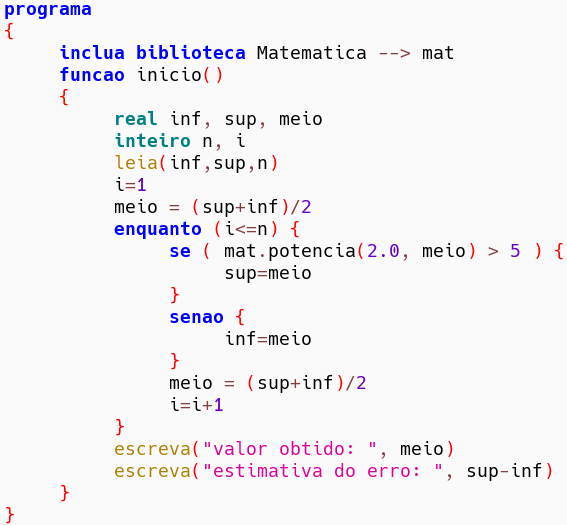
\includegraphics[width=.7\linewidth]{p2_bisseccao_2}
\end{figure}

Note que no final, o algoritmo mostra não apenas o valor obtido, como também a diferença entre os valores inferior e superior do intervalo. Essa diferença representa uma estimativa para o erro da aproximação. Dizemos estimativa porque não sabemos qual é o número que estamos procurando para calcularmos o erro de fato, sabemos apenas que ele certamente se encontra dentro de um determinado intervalo.

Usando esse algoritmo com os valores inferior e superior sempre iguais a 2 e 3, mas variando o número de repetições, obtemos os seguintes resultados:

\begin{texto}
{
	Quanto resultados possuem muitas casas decimais, o Portugol usa uma notação equivalente à científica, como essa: $9{,}765625E-4$. O significado dessa notação é $9{,}765625\cdot^10{-4}$.
}
\end{texto}

\begin{table}[H]
\centering

\begin{tabular}{|*{3}{c|}}
\hline
\tcolor{Número de repetições} & \tcolor{Valor obtido} & \tcolor{Estimativa do erro} \\
\hline
$5$ & $2{,}328125$ & $0{,}03125$ \\
\hline
$10$ & $2{,}32177734375$ & $0{,}0009765625$ \\
\hline
$20$ & $2{,}3219285011291504$ & $0{,}0000009536743$ \\
\hline
\end{tabular}
\end{table}

Note que com 5 repetições, a diferença entre os valores mínimo e máximo que delimitam o intervalo onde sabemos que está o valor analisado é igual a $0{,}03125$. Isso significa que a primeira casa decimal desses dois valores são iguais e, portanto, temos certeza de que a primeira casa depois da vírgula da representação decimal do número $\log_25$ é 3 e que, portanto, poderíamos usar a aproximação $2{,}3$ tendo certeza de que esses algarismos estão corretos.

Quando consideramos os resultados depois de $10$ repetições, já podemos fazer essa afirmação para as $3$ primeiras casas depois da vírgula, ou seja, já temos certeza de que a representação decimal do número $\log_25$ começa com $2{,}321$. De fato, note que a quarta casa decimal obtida com $10$ repetições é diferente do valor obtido com $20$ repetições.

Com $20$ repetições, já temos certeza sobre as $6$ primeiras casas depois da vírgula!

Se o nosso foco é determinar uma certa quantidade de casas decimais do número em questão, poderíamos alterar o algoritmo de modo que ele realizasse repetições até que tenhamos certeza sobre essa quantidade de casas decimais. Para isso, bastaria usar a diferença entre os valores mínimo e máximo do intervalo como critério da repetição.

Com 50 repetições, algo que é feito quase que instantaneamente com esse algoritmo em um computador convencional, estaríamos chegando no limite que o próprio Portugol consegue registrar, afinal, o computador também tem limitações na representação de números decimais. Porém, com linguagens de programação especificamente criadas para processamento numérico de alta precisão, esse processo poderia ser repetido um número muito maior de vezes.

\explore{Quantas caras?}
\label{comp-exp8}
\begin{texto}
{
Nesta seção propomos um jogo com moedas e discutimos como construir um simulador em Portugol para o jogo. Com esse simulador, não apenas os estudantes poderão simular muitas jogadas e analisar os resultados obtidos, mas também explorar pequenas variações do jogo de forma empírica. Essa abordagem pode ser interessante tanto para motivar os estudos de probabilidades teóricas quanto para verificá-los empiricamente.

A proposta desta seção dialoga diretamente com o PARA SABER MAIS proposto no final do módulo de Probabilidade, onde os autores sugerem a simulação do lançamento de uma moeda com o auxílio de planilhas eletrônicas. O que faremos aqui é análogo ao que foi feito nas planilhas, mas em uma linguagem de programação trocamos o ato de arrastar o conteúdo de uma célula para baixo por um comando de repetição (como o "\texttt{enquanto}"{} em Portugol), e os comandos "\texttt{NúmeroAleatório}"{} e "\texttt{ContarSe}"{} pelos comandos "\texttt{sorteia}"{} e "\texttt{se}". Cada abordagem traz vantagens e desvantagens e contrastá-las pode ajudar no desenvolvimento do pensamento computacional dos seus estudantes.

\textbf{Habilidades}: \textbf{EM13MAT405} (Utilizar conceitos iniciais de uma linguagem de programação na implementação de algoritmos escritos em linguagem corrente e/ou matemática) e \textbf{EM13MAT511} (Reconhecer a existência de diferentes tipos de espaços amostrais, discretos ou não, e de eventos, equiprováveis ou não, e investigar implicações no cálculo de probabilidades).

}
\end{texto}

\subsection{Usando o computador para jogar moedas}

Conta-se que um matemático foi feito prisioneiro durante a segunda guerra mundial e, para manter a mente ocupada no cárcere, lançou uma moeda $10$ mil vezes obtendo uma das faces $5067$ vezes e a outra $4933$.\footnote{Aqui seria legal uma imagem (com função meramente ilustrativa) de uma pessoa fazendo aquela contagem de risquinhos na parede típica de prisioneiros, só que dessa vez em duas colunas indicando cara e coroa e algumas moedas jogadas no chão}

A fascinação dos matemáticos que estudam probabilidade por moedas deve-se, provavelmente, ao fato de que este objeto simples (que admite apenas 2 resultados, ambos com a mesma probabilidade de ocorrência) permite a simulação de situações mais complexas e generalizantes.

Nesta seção, vamos ver como utilizar a linguagem Portugol para simular o lançamento de moedas. Nosso objetivo é criar um simulador para a seguinte questão:

\textbf{Quantas caras}? Duas moedas são lançadas e conta-se quantas caras foram obtidas a cada lançamento. Sendo assim, os resultados possíveis são: $0$, $1$ ou $2$. Antes de as moedas serem lançadas, você escolhe em qual possibilidade quer apostar. Se acertar, vence. Se errar, perde.

\begin{sugestions}{Para refletir}
{Essa discussão antes da realização das atividades é muito importante para salientar a relevância das simulações e dos cálculos das probabilidades teóricas como ferramentas que nos permitem ir além das nossas intenções (muitas vezes errôneas quando se trata de probabilidades).}
{1}{1}
\end{sugestions}
\begin{objectives}{Jogando moedas e contando caras}
{
Aplicar o pensamento computacional e formas sistemáticas de representação de um algoritmo para criar soluções para problemas relacionados a conteúdos matemáticos.
}{1}{1}
\end{objectives}
\begin{sugestions}{Jogando moedas e contando caras}
{
\textbf{Organização da turma}: sugerimos a divisão da turma em grupos pequenos ou duplas, de acordo com a disponibilidade de computadores.

\textbf{Enriquecimento da discussão}: você pode finalizar essa aula discutindo os resultados da turma, ou seja, aqueles obtidos ao agregar os resultados de todos os grupos. Com isso, seu resultado deve estar mais próximo da proporção esperada. Discuta a ocorrência de resultados diferentes entre os grupos e a importância de agregar uma quantidade maior de repetições para aumentar a confiabilidade dos resultados observados.
}{1}{2}
\end{sugestions}
\begin{answer}{Jogando moedas e contando caras}
{
\begin{enumerate}[left=1.5em]
\item[\titem{a)} e \titem{b)}] Espera-se que o resultado mais frequente seja $1$ cara, mas como o número de repetições foi baixo também é esperado que alguns grupos observem resultados diferentes.

\setcounter{enumi}{2}
\item Como os estudantes não sabem como realizar sorteios em Portugol, sugerimos que o uso de expressões mais informais (como "jogue uma moeda"{} ou "observe o resultado") seja incentivado. O importante aqui é que o estudante note que o resultado do jogo não é "cara"{} ou "coroa", mas sim a quantidade de caras observadas e isso deve ser registrado adequadamente. Tenha em mente a tabela pedida na questão \titem{b)} e o algoritmo obtido na próxima atividade.
\end{enumerate}
}{1}
\end{answer}

\begin{reflection}
Em um primeiro olhar, algum dos três resultados parece ter maior probabilidade de ocorrer? Porquê?
\end{reflection}

Vamos começar simulando o problema sem computador e depois resolveremos algumas atividades auxiliares que irão nos ajudar a finalmente construir o simulador para o jogo "Quantas caras?".

\begin{task}{Jogando moedas e contando caras}
\begin{enumerate}
\item Usando duas moedas, faça 20 lançamentos e anote os resultados em uma tabela como a mostrada abaixo.

\begin{table}[H]
\centering

\begin{tabular}{|*{3}{c|}}
\hline
\tcolor{Jogada} & \tcolor{Faces obtidas} & \tcolor{Quantas caras?} \\
\hline
$1$ & Cara-Cara & $2$ \\
\hline
$2$ & & \\
\hline
$3$ & & \\
\hline
$\vdots$ & & \\
\hline
\end{tabular}
\end{table}

\item Considerando as suas jogadas, qual foi o resultado mais frequente?

Embora você tenha feito $20$ jogadas, essa quantidade ainda é muito pequena para tirarmos conclusões sobre qual das possibilidades tem maior probabilidade de ocorrer. Podemos reunir os dados da turma toda, o que nos renderia um conjunto de dados bem maior, mas poderíamos obter ainda mais repetições desse experimento aleatório com o auxílio de um computador que simule as jogadas e anote os resultados para nós.

Então, vamos começar a pensar em como o processo de fazer várias jogadas poderia ser transformado em um algoritmo.

\item Descreva textualmente um algoritmo que realize $n$ repetições do jogo "Quantas caras?"{} e registre quantas vezes saíram $2$ caras, $1$ cara ou $0$. Não se preocupe com comandos específicos de Portugol ainda, apenas com a ideia geral do que deve ser realizado em cada etapa.
\end{enumerate}
\end{task}

\arrange{Usando o computador para jogar moedas}
\label{comp-arr8}

Agora vamos analisar o algoritmo abaixo, escrito em Portugol. Este algoritmo não simula o jogo "Quantas caras?", mas sim um experimento mais simples: jogar uma moeda e anotar a face obtida. É importante compreendê-lo bem, pois todos os elementos que precisaremos para simular o jogo "Quantas caras?"{} (e tantos outros jogos aleatórios envolvendo moedas e dados) estão presentes nele.

\begin{figure}[H]
\centering

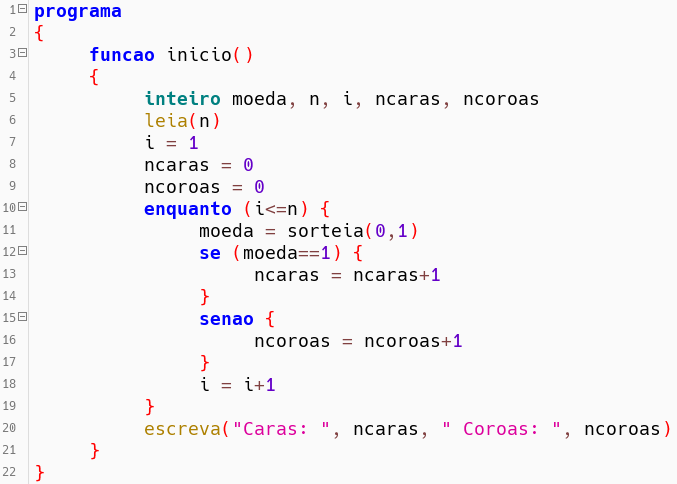
\includegraphics[width=.65\linewidth]{p2_quantascaras_1}
\end{figure}

Há um comando novo no algoritmo acima.

O comando "\verb|sorteia(x,y)|"{} seleciona aleatoriamente um número inteiro no intervalo de $x$ a $y$ (incluindo os próprios $x$ e $y$), de modo que cada valor tem a mesma chance de ser sorteado. No nosso caso, o comando da linha \verb|11| seleciona o número $0$ ou o número $1$, com $50\% $de chance de cada um deles ser selecionado.

Um último aspecto que vale a pena salientar é a interpretação do valor numérico sorteado como cara ou coroa. Isso é feito pelos comandos se e senao. Nesse caso, o algoritmo está considerando que o valor $1$ é cara e o valor 0 é coroa, mas isso pode ser definido da forma mais conveniente para os seus objetivos.

\explore{Simulando o jogo Quantas caras?}
\label{comp-exp9}
\begin{objectives}{Simulando o jogo "Quantas caras?"}
{
Aplicar o pensamento computacional e formas sistemáticas de representação de um algoritmo para criar soluções para problemas relacionados a conteúdos matemáticos.
}{1}{1}
\end{objectives}
\begin{sugestions}{Simulando o jogo "Quantas caras?"}
{
\textbf{Duração}: 1 aula no laboratório de informática.

\textbf{Organização da turma}: sugerimos a divisão da turma em grupos pequenos ou duplas, de acordo com a disponibilidade de computadores.

\textbf{Enriquecimento da discussão}: uma vez compreendido como montar o simulador para o jogo proposto, não é difícil explorar variações do mesmo jogo, como o uso de mais moedas.

\textbf{Conexões}: como dito anteriormente, a atividade se baseia em um problema de probabilidade. Um detalhe importante do ponto de vista matemático é que o jogo "Quantas caras?"{} cria um experimento aleatório em que o espaço amostral não é equiprovável. A questão 5 abre a possibilidade para discussão desse aspecto.
}{1}{1}
\end{sugestions}
\begin{answer}{Simulando o jogo Quantas caras?}
{
\begin{enumerate}[wide]
\item \adjustbox{valign=t}
{
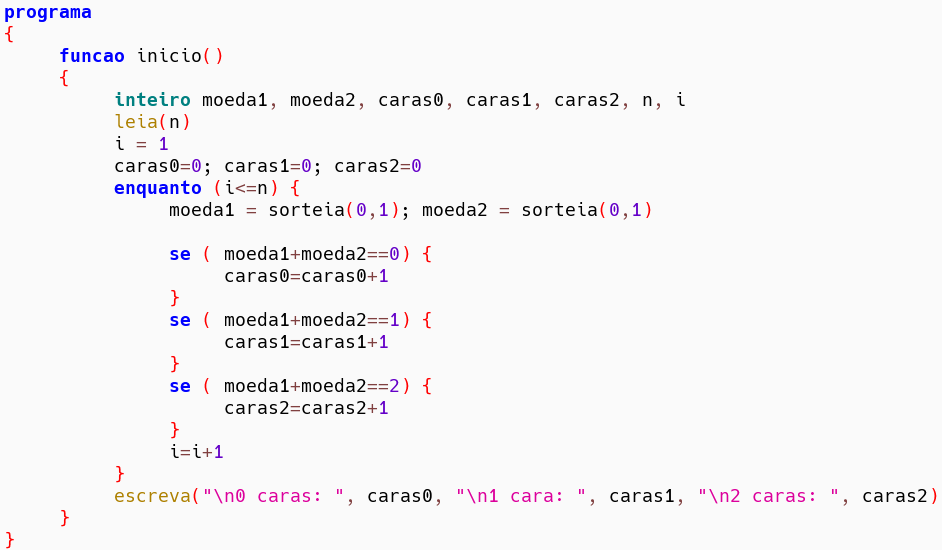
\includegraphics[width=.5\linewidth]{p2_quantascaras_2}
}
\item[\titem{b)}, \titem{c)}, \titem{d)} e \titem{e)}]
Espera-se que a frequência relativa dos resultados seja $\frac{1}{4}$, $\frac{1}{2}$ e $\frac{1}{4}$ para $2$ caras, $1$ cara e $0$, respectivamente. Na questão \titem{c)}, essas proporções devem ficar muito claras nos resultados. Essa probabilidade pode ser calculada a partir do espaço amostral de um outro experimento aleatório: lançar duas moedas e anotar as duas faces. Neste experimento, há $4$ resultados possíveis e todos equiprováveis, portanto, com probabilidade igual a $\frac{1}{4}$. Porém, um deles não apresenta caras ($0$), um deles apresenta $2$ caras e dois deles apresentam $1$ cara.
\end{enumerate}
}{1}
\end{answer}

Agora que já vimos como sortear números naturais aleatoriamente usando o Portugol, vamos criar um algoritmo que faça a simulação de quantas jogadas quisermos para o jogo "Quantas caras?".

Tudo o que você precisa para criar esse algoritmo foi apresentado anteriormente. Dois detalhes precisam ser levados em conta:

\begin{enumerate}[label=\titem{\arabic*}]
\item Duas moedas precisam ser lançadas;
\item Existem três resultados possíveis para o experimento aleatório em questão: obter 2 caras, 1 cara ou 0.
\end{enumerate}

\begin{task}{Simulando o jogo "Quantas caras?"}
\begin{enumerate}
\item Escreva um algoritmo que permita repetir o jogo "Quantas caras?"{} quantas vezes o usuário desejar.

\item Use esse algoritmo para realizar 10 jogadas. Qual dos resultados foi o mais frequente? Qual foi a frequência relativa deste resultado?

\item Use esse algoritmo para realizar 100 jogadas. Qual dos resultados foi o mais frequente? Qual foi a frequência relativa deste resultado?

\item Use esse algoritmo para realizar 10 mil jogadas. Qual dos resultados foi o mais frequente? Qual foi a frequência relativa deste resultado?

\item Repita a simulação com 10 mil jogadas algumas vezes. Considerando os resultados observados nessas simulações, qual parece ser a probabilidade de cada um dos possíveis resultados? Você concorda com essa probabilidade? Justifique.
\end{enumerate}
\end{task}

\arrange{Simulando o jogo Quantas Caras?}
\label{comp-arr9}

Você deve ter notado que os resultados obtidos na questão 5 para as frequências relativas da atividade anterior foram sempre muito próximos.

Essa estabilidade nos resultados quando consideramos a razão entre o número de caras obtidos e o número total de lançamentos é chamada de "lei dos grandes números". Essa lei, que foi apresentada no módulo sobre Probabilidade, é uma das mais importantes da estatística e diz que quando realizamos um número muito grande de repetições, a frequência observada de cada resultado se aproxima da probabilidade teórica.

O uso de computadores para realizar muitas repetições de um experimento aleatório permite-nos observar essa lei em funcionamento e pode ajudar-nos a ter uma verificação empírica dos cálculos de probabilidade que já realizamos ou indicar tendências para probabilidades que ainda não tenhamos compreendido do ponto de vista teórico.

\know{Outros experimentos com Portugol}
\label{comp-know5}

\begin{texto}
{
Este problema pode ser usado como uma extensão da atividade proposta anteriormente ou como avaliação. Se desejar uma discussão mais detalhada do Jogo do Máximo (sem o uso de uma linguagem de programação) você pode conferir o software educacional \href{https://m3.ime.unicamp.br/recursos/1237}{Explorando o Jogo do Máximo} e o seu Guia do Professor.	
}
\end{texto}

O comando sorteia pode ser utilizado para realizar outros tipos de experimentos aleatórios cujo resultados sejam discretos, como lançar um dado comum. Para isso, bastaria usar o comando sorteia da seguinte maneira: \verb|sorteia(1,6)|.

Um problema que pode ser interessante investigar empiricamente com essa ferramenta é o Jogo do Máximo: a cada jogada, dois dados comuns são lançados. Se a maior face obtida for $5$ ou $6$, o jogador $A$ vence. Se a maior face for $1$, $2$, $3$ ou $4$, o jogador $B$ vence.

\begin{figure}[H]
\centering

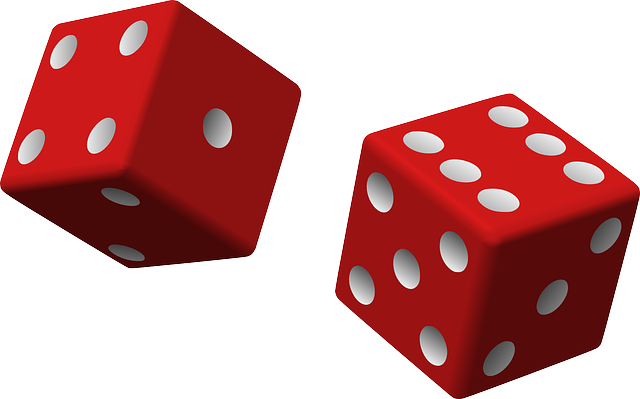
\includegraphics[width=.5\linewidth]{p2_quantascaras_3}
\caption{Imagem de Clker-Free-Vector-Images por \href{https://pixabay.com/pt/?utm_source=link-attribution\&utm_medium=referral\&utm_campaign=image\&utm_content=25637}{Pixabay}}
\label{}
\end{figure}

A pergunta a ser investigada é: qual dos dois jogadores tem maior probabilidade de vencer?


\explore{Tem sinal?}
\label{comp-exp10}
\begin{texto}
{
Nesta seção, propomos um problema que lida com inequações não lineares, coordenadas de pontos no plano cartesiano, circunferência e distância entre pontos,. Esse problema se traduz em detectar se um ponto está dentro de uma circunferência e o objetivo final da seção é que os estudantes criem um algoritmo que faça essa verificação para um ponto e um número grande de "torres". Dessa forma, a seção oferece uma aplicação atual de vários conceitos, conectando-os via criação de um algoritmo em Portugol.

Do ponto de vista computacional, utilizamos repetições e alguns cálculos. Também introduzimos os conceitos de "entrada"{} (as informações que são dadas a um algoritmo para que ele execute suas ações) e "saída"{} (as informações que ele gera ao longo de sua execução).

A nossa sugestão é que esta seção seja utilizada após os estudos do módulo sobre Sistemas Lineares e Inequações. Os dois \textbf{Organizando} que compõem esta seção trazem uma discussão breve relacionada a esses conteúdos, que você pode estender e aprofundar se desejar.

\textbf{Habilidades}: \textbf{EM13MAT405} (Utilizar conceitos iniciais de uma linguagem de programação na implementação de algoritmos escritos em linguagem corrente e/ou matemática).
}
\end{texto}
\clearmargin
\begin{objectives}{Tem sinal? - parte 1}
{
Compreender como sistematizar soluções algorítmicas através de recursos como a linguagem matemática, fluxogramas ou linguagens de programação.


}{1}{2}
\end{objectives}
\begin{sugestions}{Tem sinal? - parte 1}
{
\textbf{Recomendações gerais}: esta atividade foi concebida para uso em sala de aula.

\textbf{Duração}: 1 aula, incluindo a discussão do Organizando logo em seguida.

\textbf{Organização da turma}: a atividade pode ser feita idividualmente ou em pequenos grupos.

\textbf{Conexões}: esta atividade, na verdade, lida principalmente com conteúdos matemáticos ligados à Geometria Analítica (ponto, circunferência e distância entre pontos) e Álgebra (inequações). É recomendável que você aproveite o contexto para relembrar esses conceitos.


}{1}{2}
\end{sugestions}
\begin{answer}{Tem sinal? - parte 1}
{
\begin{enumerate}
\item Sim.

\item Não.

\item O que buscamos aqui é que os estudantes percebam que basta verificar se a distância do ponto ao centro da circunferência é menor do que o raio.

\item O que buscamos aqui é uma descrição que remeta à fórmula para cálculo da distância entre dois pontos no plano cartesino. Porém, não há necessidade de usar a fórmula fechada se o estudante souber descrever o processo usando a diferença entre as coordendas e o Teorema de Pitágoras.

\item O ponto está dentro do alcance da torre.
\end{enumerate}
}{1}
\end{answer}

Hoje em dia, a disponibilidade de sinal de celular é uma questão que vai além do acesso a redes sociais ou entretenimento. Com o aumento do uso da internet em diferentes áreas, ter acesso à internet pode ser determinante para que tenhamos acesso a serviços de saúde, educação, bancário, etc.

Nesta seção, vamos investigar, com o auxílio do computador, um problema relacionado à disponibilidade de sinal em uma determinada localidade.

O cenário que vamos adotar aqui é uma pequena simplificação do que acontece na realidade. Vamos considerar posições dadas em um plano cartesiano (com eixos dados em quilômetros) e que algum tipo de sinal é emitido radialmente por torres. A posição dessas torres também é dada por coordenadas no plano e cada torre possui um alcance diferente, como mostrado abaixo.

\begin{figure}[H]
\centering

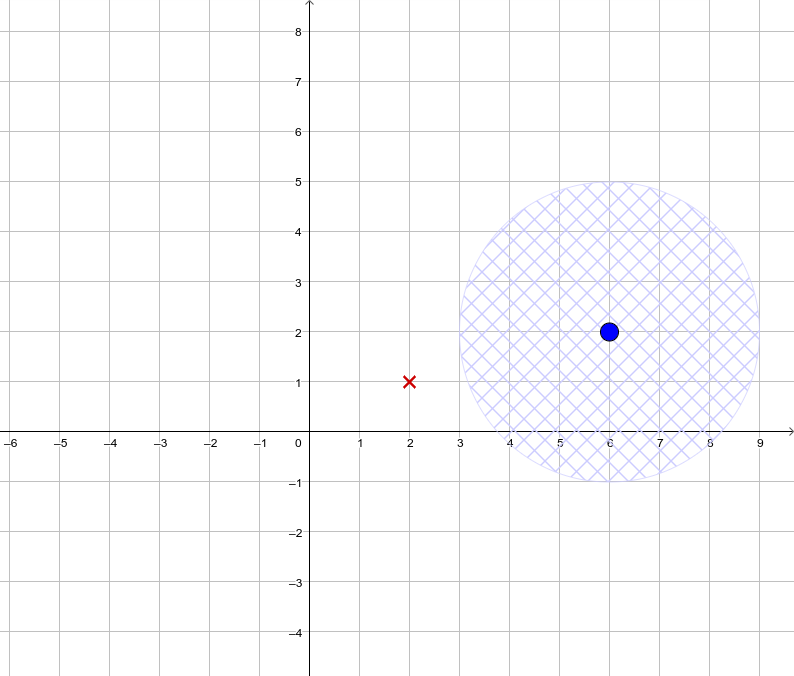
\includegraphics[width=.75\linewidth]{p2_sinal_1}
\end{figure}

Por exemplo, na imagem acima, o aparelho celular está na posição marcada com x, que tem coordendas $(2;1)$ e a torre está na posição $(6;2)$ e tem um alcance de $3$ quilômetros.

Quando temos uma representação visual em mãos, é fácil dizer se um ponto dado está dentro do alcance de uma torre dada. No caso acima, a resposta é não. Mas e quando temos apenas as coordenadas do celular e da torre?

\clearpage

\begin{task}{Tem sinal? - parte 1}
\begin{enumerate}
\item Considere que uma nova torre com alcance de $3$ quilômetros foi instalada no ponto de $(1;-1)$. Represente essa nova torre e o seu alcance na imagem acima. O ponto $x$ está dentro do alcance dessa nova torre?

\item Considere agora que uma terceira torre com alcance de $4$ quilômetros foi instalada no ponto de $(-1;4)$. Represente essa nova torre e o seu alcance na imagem acima. O ponto $x$ está dentro do alcance dessa nova torre?

Por mais que a sua representação tenha sido feita com cuidado, é possível que você tenha ficado com dúvidas sobre a resposta para a questão \titem{b)}, não?

\item Como podemos decidir, a partir das coordenadas da posição do celular e das torres em seu entorno, se o ponto $x$ está dentro do alcance de cada uma das torres?

Embora possa haver limitações em termos de precisão ou de dificuldade em desenhar, nós podemos usar representações visuais para resolver questões, especialmente as que envolvem objetos geométricos. Porém, computadores não contam com esse recurso. De maneira geral, objetos geométricos são tratados por meio de suas coordendas e questões como essa (se um ponto está dentro ou fora de uma circunferência) são respondidas com o auxílio de alguns cálculos.

\item Descreva textualmente como proceder para determinar se um ponto no plano está dentro ou fora de uma circunferência dadas as coordenadas do ponto, as coordenadas do centro da circunferência e o seu raio. Sua descrição deve contemplar todos os passos da resolução e ser aplicável a quaisquer pontos e torres.

\item Aplique a sua descrição para o caso em que o ponto está na posição $(0;-2)$ e a torre foi instalada na posição $(1;-4)$ e tem alcance de $5$ quilômetros.
\end{enumerate}
\end{task}

\arrange{Soluções para inequações}
\label{comp-arr10}

Ao responder a pergunta "um ponto dado está dentro do alcance de pelo menos uma das  torres dadas?", estamos lidando com um conjunto de  inequações e isso é diferente do que fazemos quando lidamos com sistemas de equações lineares, por alguns motivos, como vemos a seguir.

Primeiro, não estamos lidando com equações, mas sim inequações. Neste contexto, as equações correspondem às linhas que delimitam o alcance da torre, enquanto que as inequações correspondem ao círculo que demarca toda a região alcançada pela torre (ou a parte de fora desse círculo se invertermos o sinal de desigualdade).

Segundo, as equações envolvidas não são lineares pois as circunferências são dadas por equações que têm as variáveis  e  elevadas ao quadrado .

Terceiro, e mais importante, não estamos buscando uma solução para o sistema de inequações. Isso significaria encontrar as coordenadas de um ponto satisfazendo todas elas. O que nos interessa é se o ponto é solução de pelo menos uma das inequações.

\begin{figure}[H]
\centering

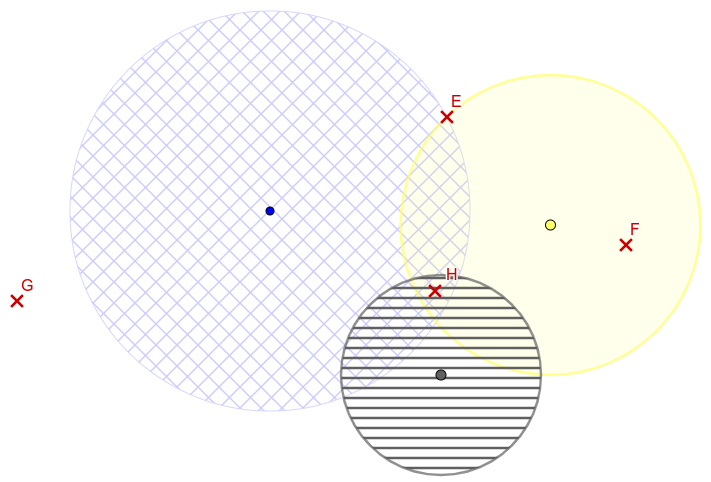
\includegraphics[width=.75\linewidth]{p2_sinal_2}
\end{figure}

Na figura acima, o ponto $H$ é uma solução das três inequações que determinam os três círculos mostrados. O ponto $E$ é solução de duas das equações que determinam as circunferências traçadas. Já o ponto $F$ é solução de apenas uma das inequações que determinam os círculo e o ponto $G$ não é solução de nenhuma dessas inequações.

Considerando esses quatro pontos, em qual deles há sinal?

\explore{Tem sinal? - parte 2}
\label{comp-exp11}
\begin{objectives}{Tem sinal? - parte 2}
{
Compreender como sistematizar soluções algorítmicas através de recursos como a linguagem matemática, fluxogramas ou linguagens de programação.
}{1}{1}
\end{objectives}
\begin{sugestions}{Tem sinal? - parte 2}
{
\textbf{Comentários gerais}: esta atividade foi concebida para uso em laboratório. Por ser a última atividade do módulo, não sugerimos a resolução em fluxograma primeiro, mas você pode incluir essa etapa se julgar adequado logo antes da questão 1.

\textbf{Duração}: 1 aula.

\textbf{Dificuldades}: tenha certeza de que os estudantes leram e compreenderam o que foi apresentado no Explorando que antecede a atividade, pois ele deve esclarecer pontos potencialmente difíceis. A descrição da entrada esperada para o algoritmo é uma novidade desta atividade. Apesar de incomum, não é difícil compreendê-la: ela apenas descreve a ordem em que os comandos "leia"{} devem ser usados.
}{1}{1}
\end{sugestions}
\begin{answer}{Tem sinal? - parte 2}
{

\begin{enumerate}
\item \adjustbox{valign=t}
{
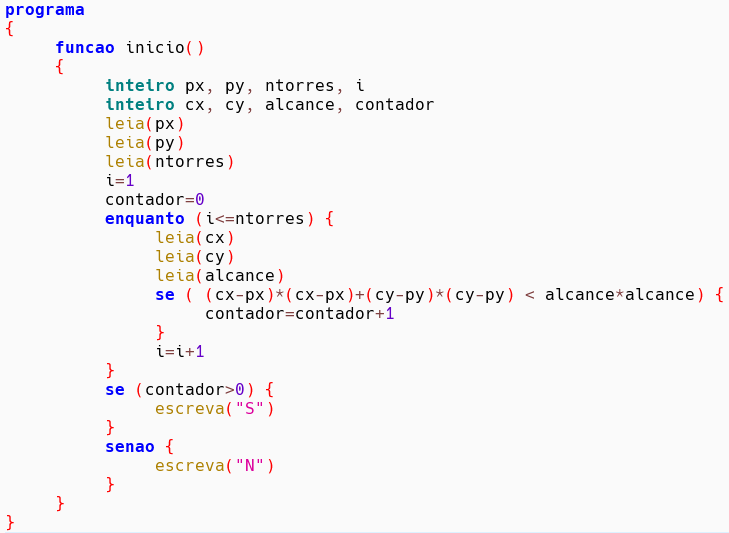
\includegraphics[width=.8\linewidth]{p2_sinal_4.png}
}

\item Os testes estão todos corretos. Você pode sugerir que os estudantes criem novos casos, testem com seus algoritmos e depois troquem entre si.
\end{enumerate}
}{1}
\end{answer}

Agora que você já sabe como resolver esse problema a partir das coordendadas dos pontos envolvidos, podemos utilizar essa abordagem para criar um algoritmo que diga se há sinal em um ponto a partir das informações de várias torres.

Mas antes de começar a implementar a solução em Portugol, vejamos alguns detalhes da linguagem que pode afetar a sua solução:

\begin{itemize}
\item Para elevar um número ao quadrado ou extrair a sua raiz quadrada, você vai precisar usar comandos que não fazem parte das funcionalidades básicas do Portugol, mas estão disponíveis como parte de uma biblioteca chamada Matematica. Isso é simples, e de fato está explicado na seção sobre o método da bissecção ou pode ser entendido com auxílio \href{https://www.youtube.com/watch?v=rs8ihN08bgU&feature=youtu.be}{deste vídeo}. Mas para evitar esses pontos, podemos simplesmente usar o fato de que $x^=x\cdot x$;
\item Os símbolos de desigualdades disponíveis em Portugol são: \verb|<| (menor que), \verb|>| maior que, \verb|<=| (menor ou igual a) e \verb|>=| (maior ou igual a)
\end{itemize}

\begin{task}{Tem sinal? - parte 2}
Nesta atividade, você deve escrever um algoritmo que leia as informações a partir de um formato específico. Primeiro, o usuário irá digitar as coordenadas $x$ e $y$, nessa ordem, do ponto para o qual vamos analisar a existência de sinal. Esses dois valores devem ser variáveis inteiras. Depois, um número inteiro referente ao número de torres que serão consideradas. Por fim, para cada torre serão dados três valores (todos reais) representando a sua coordenada $x$, coordenada $y$ e alcance. Segue um exemplo explicado:


\begin{table}[H]
\centering

\begin{tabular}{>{\ttfamily\catcode`_=12}c >{\em}l}
2 &   (coordenada $x$ do ponto) \\
-1 & (coordenada $y$ do ponto) \\
3  & (quantidade de torres) \\
-10 & (coordenada $x$ da torre 1) \\
3  & (coordenada $y$ da torre 1) \\
6  & (alcance da torre 1) \\
7  & (coordenada $x$ da torre 2) \\
6  & (coordenada $y$ da torre 2) \\
4  & (alcance da torre 2) \\
10 & (coordenada $x$ da torre 3) \\
1 &  (coordenada $y$ da torre 3) \\
7  & (alcance da torre 3) \\
\end{tabular}
\end{table}



A resposta do seu algoritmo deve ser um único caractere: \verb|S| ou \verb|N|, se houver ou não sinal no ponto dado. No caso do exemplo dado, a saída deve ser: \verb|N|

\begin{enumerate}
\item Escreva um algoritmo em Portugol que resolva o problema proposto seguindo o formato de entrada descrito acima.

Você pode usar o exemplo acima para testar a sua solução.

\item A seguir estão disponíveis mais alguns casos para você testar com o seu algoritmo.

\begin{table}[H]
\centering

\begin{tabular}{|*{3}{>{\ttfamily\catcode`_=12} c|}}
\hline
\verb|Entrada| & \verb|Entrada| & \verb|Entrada| \tabularnewline
0 & -1 & 2 \tabularnewline
0 & 1 & -1 \tabularnewline
2 & 1 & 4 \tabularnewline
3 & -5 & 10 \tabularnewline
3 & 1 & 10 \tabularnewline
4 & 5 & 10 \tabularnewline
-2 & Saída & -2 \tabularnewline
-2 & N & -2 \tabularnewline
3 & & 4 \tabularnewline
Saída & & 0 \tabularnewline
S & & 6 \tabularnewline
& & 7 \tabularnewline
& & 1 \tabularnewline
& & -5 \tabularnewline
& & 5 \tabularnewline
& & Saída \tabularnewline
& & N \tabularnewline
\hline
\end{tabular}
\end{table}
\end{enumerate}
\end{task}

\arrange{Regiões no plano}
\label{comp-arr11}

Você estudou no módulo sobre sistemas lineares o significado geométrico da resolução de sistemas de equações lineares: equações lineares determinam retas e a solução de sistemas com duas ou mais equações lineares determinam os pontos de intersecção entre essas retas. Resolver uma inequação significa, geometricamente, encontrar os pontos de um intervalo ou região que satisfazem essa inequação. Portanto, resolver um sistema de inequações significa encontrar os pontos que estejam localizado na sobreposição (ou intersecção) de todas as regiões determinadas por cada uma das inequações.

Uma inequação linear de duas variáveis determina um semi-plano e um sistema de inequações lineares determina regiões que resultam da sobreposição desses semiplanos, podendo ser usados para determinar a parte interior de um polígono, por exemplo. Seguindo esse raciocínio, o interior de um pentágono poderia ser dado por um sistema de 5 inequações lineares e é possível checar se um ponto está dentro do pentágono verificando se as coordenadas do ponto satisfazem todas a inequações. Porém, essa é apenas uma das maneiras de fazer essa checagem para o caso de um polígono. Com ferramentas que você poderá estudarno Ensino Superior, mais especificamente no curso de Geometria Analítica, outros métodos estarão disponíveis.

Relembrando que o problema que resolvemos aqui não pretendia verificar se um ponto satisfaz um sistema de inequações, mas sim se ele satisfaz pelo menos uma das inequações de um conjunto de inequações.


\know{A Olimpíada Brasileira de Informática}
\label{comp-know6}

Você talvez não saiba, mas ao longo das seções deste módulo você resolveu várias questões que fizeram parte da Olimpíada Brasileira de Informática. Alguns exemplos são os problemas Cometa, Conteineres, Xadrez e Campeonato.

\begin{figure}[H]
\centering

\includegraphics[width=.6\linewidth]{p2_sinal_3.jpg}
\end{figure}

Nessa olimpíada, os participantes devem resolver 3 ou 4 problemas em um período de tempo delimitado e submeter as suas soluções, que são pontuadas automaticamente. O sistema usado para isso depende de instruções muito rígidas para a entrada e saída de cada algoritmo a ser resolvido, mas agora que você aprendeu sobre isso e já conhece os conceitos básicos de uma linguagem de programação, pode participar dessa competição!

Todos os problemas já propostos nessa olimpíada estão disponíveis em \url{olimpiada.ic.unicamp.br/pratique}, organizados por ano, nível e fase. Além disso, o sistema de correção de todos eles está disponível para que você possa testar as suas próprias soluções.

Infelizmente, a OBI não aceita algoritmos escritos em Portugol, mas ela oferece alguns materiais de estudo alinhados ao estilo da competição em \url{olimpiada.ic.unicamp.br/estude}. São referências muito boas para quem deseja aprender mais sobre programação de computadores, mesmo que não planeje participar da olimpíada.


\ifnum\aluno=1
\clearpage
\else
\notasfinais
\fi

\bibliographystyle{apalike-pt}
\bibliography{../Bibliografia/computacional_bibliografia.bib}

\nocite{*}